% \documentclass[journal]{vgtc}                % final (journal style)
\documentclass{vgtc}         % review (journal style)
%\documentclass[widereview]{vgtc}             % wide-spaced review
%\documentclass[preprint,journal]{vgtc}       % preprint (journal style)

%% Uncomment one of the lines above depending on where your paper is
%% in the conference process. ``review'' and ``widereview'' are for review
%% submission, ``preprint'' is for pre-publication, and the final version
%% doesn't use a specific qualifier.

%% Please use one of the ``review'' options in combination with the
%% assigned online id (see below) ONLY if your paper uses a double blind
%% review process. Some conferences, like IEEE Vis and InfoVis, have NOT
%% in the past.

%% Please use the ``preprint''  option when producing a preprint version
%% for sharing your article on an open access repository

%% Please note that the use of figures other than the optional teaser is not permitted on the first page
%% of the journal version.  Figures should begin on the second page and be
%% in CMYK or Grey scale format, otherwise, colour shifting may occur
%% during the printing process.  Papers submitted with figures other than the optional teaser on the
%% first page will be refused. Also, the teaser figure should only have the
%% width of the abstract as the template enforces it.

%% These few lines make a distinction between latex and pdflatex calls and they
%% bring in essential packages for graphics and font handling.
%% Note that due to the \DeclareGraphicsExtensions{} call it is no longer necessary
%% to provide the the path and extension of a graphics file:
%% \includegraphics{diamondrule} is completely sufficient.
%%
\ifpdf%                                % if we use pdflatex
  \pdfoutput=1\relax                   % create PDFs from pdfLaTeX
  \pdfcompresslevel=9                  % PDF Compression
  \pdfoptionpdfminorversion=7          % create PDF 1.7
  \ExecuteOptions{pdftex}
  \usepackage{graphicx}                % allow us to embed graphics files
  \DeclareGraphicsExtensions{.pdf,.png,.jpg,.jpeg} % for pdflatex we expect .pdf, .png, or .jpg files
\else%                                 % else we use pure latex
  \ExecuteOptions{dvips}
  \usepackage{graphicx}                % allow us to embed graphics files
  \DeclareGraphicsExtensions{.eps}     % for pure latex we expect eps files
\fi%
\usepackage{multirow}%to make table with many lines
%% it is recomended to use ``\autoref{sec:bla}'' instead of ``Fig.~\ref{sec:bla}''
\graphicspath{{../figures/}{pictures/}{images/}{./}} % where to search for the images
\usepackage{float}
\usepackage{microtype}                 % use micro-typography (slightly more compact, better to read)
\PassOptionsToPackage{warn}{textcomp}  % to address font issues with \textrightarrow
\usepackage{textcomp}                  % use better special symbols
\usepackage{mathptmx}                  % use matching math font
\usepackage{times}                     % we use Times as the main font
\renewcommand*\ttdefault{txtt}         % a nicer typewriter font
\usepackage{cite}                      % needed to automatically sort the references
\usepackage{tabu}                      % only used for the table example
\usepackage{booktabs}                  % only used for the table example
\usepackage{hyperref}
\usepackage{amssymb}
\usepackage{mathtools}
%% We encourage the use of mathptmx for consistent usage of times font
%% throughout the proceedings. However, if you encounter conflicts
%% with other math-related packages, you may want to disable it.

%% In preprint mode you may define your own headline. If not, the default IEEE copyright message will appear in preprint mode.
%\preprinttext{To appear in IEEE Transactions on Visualization and Computer Graphics.}

%% In preprint mode, this adds a link to the version of the paper on IEEEXplore
%% Uncomment this line when you produce a preprint version of the article 
%% after the article receives a DOI for the paper from IEEE
%\ieeedoi{xx.xxxx/TVCG.201x.xxxxxxx}

%% If you are submitting a paper to a conference for review with a double
%% blind reviewing process, please replace the value ``0'' below with your
%% OnlineID. Otherwise, you may safely leave it at ``0''.
\onlineid{1001}

%% declare the category of your paper, only shown in review mode
\vgtccategory{Research}
%% please declare the paper type of your paper to help reviewers, only shown in review mode
%% choices:
%% * algorithm/technique
%% * application/design study
%% * evaluation
%% * system
%% * theory/model
\vgtcpapertype{Application}

%% Paper title.
\title{Topological Analysis of
% Enstrophy\\in
Ensembles of Hydrodynamic Turbulent Flows\\
An Experimental Study}

%% This is how authors are specified in the journal style

%% indicate IEEE Member or Student Member in form indicated below
\author{Florent Nauleau \\
\scriptsize CEA \and Fabien Vivodtzev \\
\scriptsize CEA
\and Thibault Bridel-Bertomeu\thanks{\{firstname.lastname\}@cea.fr} \\
\scriptsize CEA
\and H\'elo\"ise Beaugendre\thanks{\{firstname.lastname\}@math.u-bordeaux.fr}\\
\scriptsize University of Bordeaux
\and Julien Tierny\thanks{\{firstname.lastname\}@sorbonne-universite.fr}\\
\scriptsize CNRS}
% /Sorbonne}
% niversit\'e}
\authorfooter{
%% insert punctuation at end of each item
\item
 Florent Nauleau, Thibault Bridel-Bertomeu and Fabien Vivodtzev are with the
CEA. E-mail: \{firstname.lastname\}@cea.fr.
\item
 H\'elo\"ise Beaugendre is with University of Bordeaux and Bordeaux INP. E-mail:
firstname.lastname@math.u-bordeaux.fr.
\item
Julien Tierny is with Sorbonne Universit\'e and CNRS. E-mail:
firstname.lastname@sorbonne-universite.fr.
}

%other entries to be set up for journal
\shortauthortitle{Biv \MakeLowercase{\textit{et al.}}: Global Illumination for Fun and Profit}
%\shortauthortitle{Firstauthor \MakeLowercase{\textit{et al.}}: Paper Title}

%% Abstract section.
\abstract{
This application paper presents a comprehensive experimental evaluation of the
suitability of Topological Data Analysis (TDA)
% topological data representations and their associated analysis
% tools
for the quantitative comparison of turbulent flows. Specifically, our
study documents the usage of the persistence diagram of the maxima of flow
enstrophy (an established vorticity indicator), for the topological representation of 180 ensemble members, generated
by a coarse sampling of the parameter space of five numerical solvers.
We document five main hypotheses reported by domain experts, describing their
expectations regarding the variability of the flows generated by the distinct
solver configurations. We contribute three evaluation protocols to assess the
validation of the above hypotheses by two comparison measures:
\emph{(i)} a standard distance used in scientific imaging (the $L_2$ norm) and
\emph{(ii)} an established topological distance between persistence diagrams
(the $L_2$-Wasserstein metric).
Extensive experiments on the input ensemble demonstrate
% overall
the
superiority of the topological distance (\emph{ii}) to report as close to each
other flows which are expected to be similar by domain experts, due to the
% number and size
configuration
of their vortices.
Overall,
% w
% we believe that
the insights reported by
our study bring an experimental evidence of the suitability
of TDA for representing and comparing turbulent flows, thereby providing
to the fluid dynamics community
confidence for its usage in future work.
% by the fluid dynamics community.
Also, our flow data and evaluation protocols provide to the TDA community an
application-approved benchmark for the evaluation and design of further
topological distances.}
%
%
% presents an experimental study about the suitability of
% topological data representations (and their associated analysis tools), for the
% interpretation of ensembles of simulated hydrodynamic turbulent flows.
% In particular, in this application, domain experts wish to compare the quality
% of a selection of five numerical solvers, under a specific selection of input
% parameters (domain resolution, interpolation scheme and order, etc).
%
% comparative
%
% while diagram capture visually the main vortices,
%
% the involved simulations are subject to a specific number of
% parameters (domain resolution, interpolation scheme and order)
%
% analysis of
% ensembles of turbulent flows.
%
%
% This is an abstract.
% %% draft draft draft
% Overall, our work provides tangible empirical evidence that the persistence
% diagram is an informative representation of vortices in turbulent flows and
% that its associated $L_2$-Wasserstein metric is relevant for the comparison of
% solver configurations, hence experimentally encouraging a widespread usage of
% topological methods for the analysis of ensembles of turbulent flow.
% draft draft draft
% } % end of abstract

%% Keywords that describe your work. Will show as 'Index Terms' in journal
%% please capitalize first letter and insert punctuation after last keyword
% \keywords{Topological data analysis, ensemble data, turbulent flow}

%% ACM Computing Classification System (CCS). 
%% See <http://www.acm.org/class/1998/> for details.
%% The ``\CCScat'' command takes four arguments.

% \CCScatlist{ % not used in journal version
%  \CCScat{K.6.1}{Management of Computing and Information Systems}%
% {Project and People Management}{Life Cycle};
%  \CCScat{K.7.m}{The Computing Profession}{Miscellaneous}{Ethics}
% }

%% A teaser figure can be included as follows
\teaser{
  \centering
  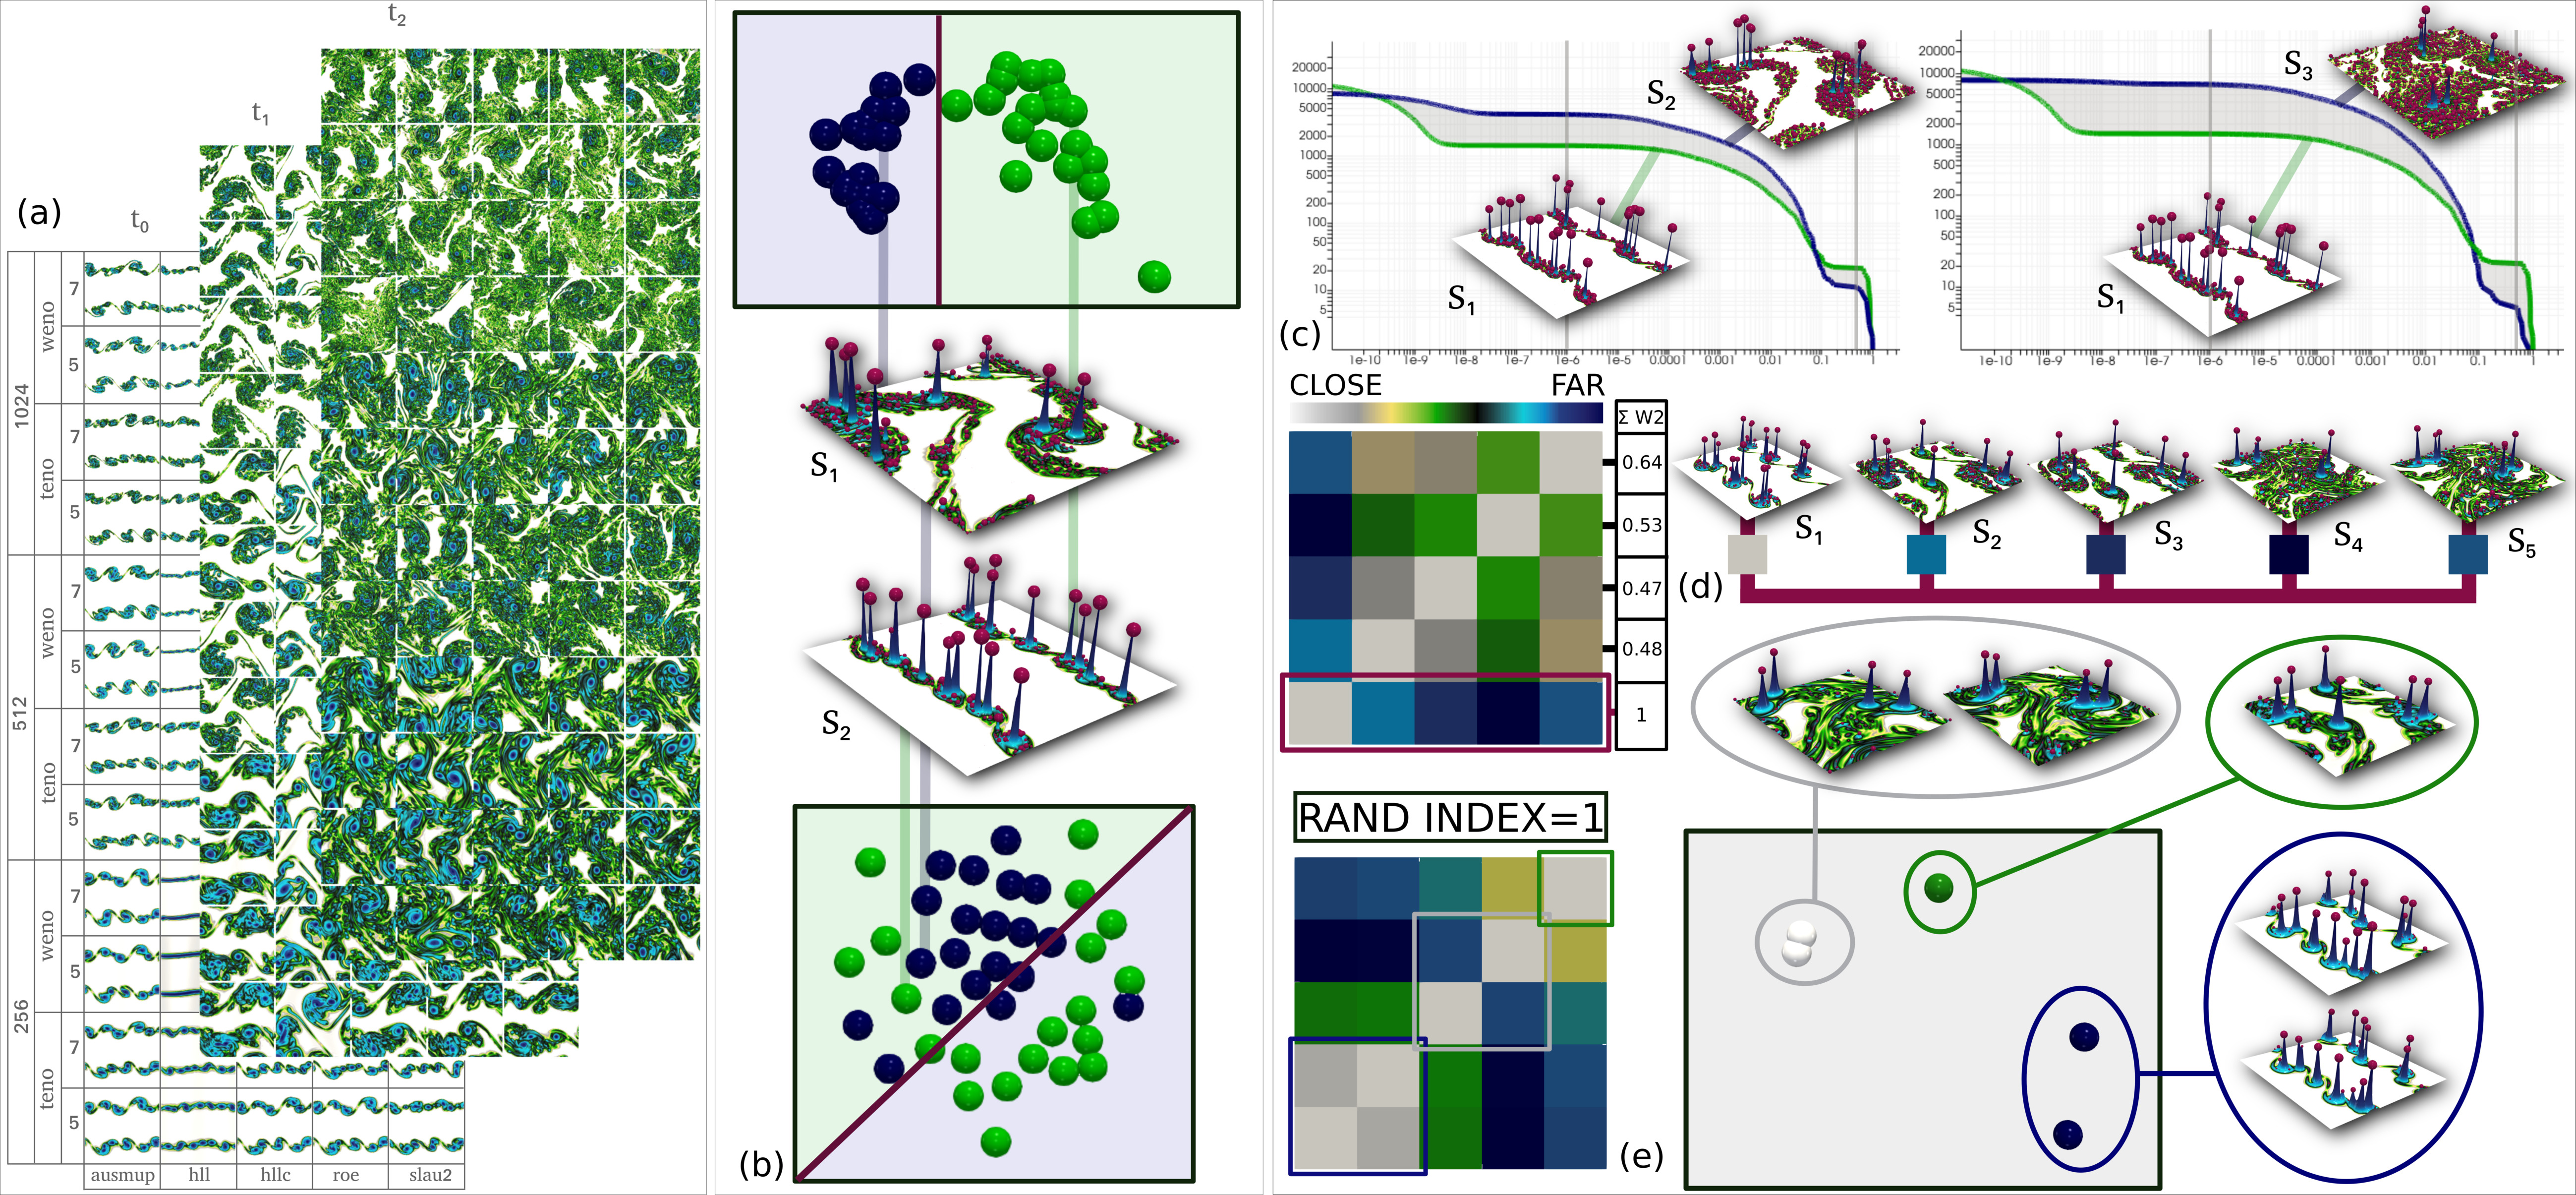
\includegraphics[width=\figureShrink\linewidth]{teaser2.jpg}
  \caption{Topological Data Analysis protocols 
%   to illustrate the segmentation 
applied
  on an ensemble dataset of a Kelvin-Helmholtz instability.
(a) The 180 members of the ensemble obtained with variations of timesteps, interpolation schemes, orders, resolutions and Riemann solvers (\autoref{tab_parameters}).
(b) The top cluster represents the time separation of $t_0$ and $t_1$ for the 
flows $S_1$ and $S_2$ with the Wasserstein distance and the bottom cluster with 
the $L_2$-norm. Red lines show the timestep separation with our clustering 
method whereas the sphere colors are the ground truth, illustrating the 
limitation of the $L_2$-norm. 
(c) \textit{Persistence curve protocol}: Differences between integrals of persistence curves (gray area) of the enstrophy computed with a SLAU2 solver, an order 7 TENO scheme and a resolution of $1024\times 1024$ for various configurations ($S_1$ at $t_0$, $S_2$ and $S_3$ at $t_1$). These integral differences exhibit the appearance of vortices (critical points) as the time increases.
(d) \textit{Outlier distance protocol}: Wasserstein distance matrix for 5 configurations $S_1(t_0,HLLC)$, $S_2(t_1,Roe)$, $S_3(t_1,HLLC)$, $S_4(t_2,Roe)$, $S_5(t_2,HLLC)$ computed with an order 7 WENO-Z interpolation scheme at $512\times 512$.
The sum of each row
% allows us to identify
the configuration maximizing this distance between solvers and timesteps, here $S_1$.
(e) \textit{Unsupervised classification}: Wasserstein distance matrix for the 
previous configurations with an order 7 WENO-Z interpolation scheme at 
$256\times 256$. The clustering based on the Wasserstein distance and colored 
according to the Kmeans clustering method successfully segments the time 
steps.}
 %Ensembles dataset of a hydrodynamic turbulence, a Kelvin Helhmotz instability at three different times, computed with two interpolation methods, with high orders, on several grids and for five Riemann solvers(\autoref{tab_parameters}).
%Maximum critical points are represented by a red sphere scaled by persistence. The two tables of points are the representation of the time separation $t_0$ and $t_1$ (Top: Wassertein distance, Bottom: L2 norm). The red line represents the ground truth of the time step separation and the colored background, the clustering obtained by our methods for the time separation. %We can see that L2 does not obtain the right cluster unlike W2 (S1 and S2). 
%  (c): Persistence curves for 2 configurations of KHI with the SLAU2 solver, the TENO scheme at order 7 on 1024 mesh for different simulation times ($S_1 and S_3$ : $t_0$, $S_2$ :$t_1$, $S_4$ :$t_2$). We can see that the number of small critical point peers is larger as a function of time than the number of large peers decreases during the simulation. The grey area represents the difference of integral between the curves. 
% (d): Wassertein distance matrix for five configurations with WENO-Z interpolations at order seven with 512 cells. $S_1$, ,$S_3$, ,$S_5$ generated with the HLLC respectively at time $t_0$, $t_1$, $t_2$. $S_2$, ,$S_4$ generated with the Roe solver respectively at time $t_1$, $t_2$. The sum of each row of the matrix is computed and normalized with respect to the KHI that maximizes the distances, here $S_1$. %We see that the case at $t_0$ is very different from the other simulations.We see that the case at $t_0$ is very different from the other simulations.(e)\textit{unsupervised classification}: Wassertein distance matrix for the 5 same configurations with an order 7 WENO-Z interpolation scheme at $256x256$.Clustering based on the Wassertein distance colored according to the Kmeans clustering method successfully segmenting the time steps.}
  \label{fig_teaser}
}

%% Uncomment below to disable the manuscript note
%\renewcommand{\manuscriptnotetxt}{}

%% Copyright space is enabled by default as required by guidelines.
%% It is disabled by the 'review' option or via the following command:
% \nocopyrightspace


\vgtcinsertpkg

%%%%%%%%%%%%%%%%%%%%%%%%%%%%%%%%%%%%%%%%%%%%%%%%%%%%%%%%%%%%%%%%
%%%%%%%%%%%%%%%%%%%%%% START OF THE PAPER %%%%%%%%%%%%%%%%%%%%%%
%%%%%%%%%%%%%%%%%%%%%%%%%%%%%%%%%%%%%%%%%%%%%%%%%%%%%%%%%%%%%%%%%



\newcommand{\lt}{<}
\newcommand{\gt}{>}

\newcommand{\discreteMorseFunction}{\mathcal{F}}
\newcommand{\discreteGradientField}{\mathcal{G}}
\newcommand{\discreteVectorField}{\mathcal{V}}
\newcommand{\dimensionality}{d}
\newcommand{\chainGroup}{\mathcal{C}}
\newcommand{\boundaryGroup}{\mathcal{B}}
\newcommand{\cycleGroup}{\mathcal{Z}}
\newcommand{\homologyGroup}{\mathcal{H}}
\newcommand{\persistentHomologyGroup}{\mathcal{PH}}
\newcommand{\domain}{\mathcal{M}}
\newcommand{\stableManifold}{\domain}
\newcommand{\unstableManifold}{\domain'}
\newcommand{\range}{\mathbb{R}}
\newcommand{\sublevelset}[1]{#1^{-1}_{-\infty}}
\newcommand{\superlevelset}[1]{#1^{-1}_{+\infty}}
\newcommand{\Star}{St}
\newcommand{\Link}{Lk}
\newcommand{\simplex}{\sigma}
\newcommand{\face}{\tau}
\newcommand{\lowerlink}{\Link^{-}}
\newcommand{\upperlink}{\Link^{+}}
\newcommand{\Index}{\mathcal{I}}
\newcommand{\offset}{o}
\newcommand{\Natural}{\mathbb{N}}
\newcommand{\criticalSet}{\mathcal{C}}
\newcommand{\diagram}{\mathcal{D}}
\newcommand{\persistentCurve}{\mathcal{C}}
\newcommand{\wasserstein}[1]{W_#1}
\newcommand{\projection}{\Delta}
\newcommand{\hierarchy}{\mathcal{H}}
\newcommand{\decimation}{D}
\newcommand{\xDimD}{L_x^\decimation}
\newcommand{\yDimD}{L_y^\decimation}
\newcommand{\zDimD}{L_z^\decimation}
\newcommand{\xDim}{L_x}
\newcommand{\yDim}{L_y}
\newcommand{\zDim}{L_z}
\newcommand{\Grid}{\mathcal{G}}
\newcommand{\GridD}{\mathcal{G}^\decimation}
\newcommand{\x}{\phantom{x}}
\newcommand{\Mod}{\;\mathrm{mod}\;}
\newcommand{\NN}{\mathbb{N}}
\newcommand{\forwardIntegralLine}{\mathcal{L}^+}
\newcommand{\backwardIntegralLine}{\mathcal{L}^-}
\newcommand{\triangulationOp}{\phi}
\newcommand{\decimationOp}{\Pi}
\newcommand{\isovalue}{w}
\newcommand{\persistence}{\mathcal{P}}
\newcommand{\pointMetric}[1]{d_#1}
\newcommand{\diagramSet}{\mathcal{S}_\mathcal{D}}
\newcommand{\diagramSpace}{\mathbb{D}}
\newcommand{\jointree}{\mathcal{T}^-}
\newcommand{\splittree}{\mathcal{T}^+}
\newcommand{\mergetree}{\mathcal{T}}
\newcommand{\mergetreeSet}{\mathcal{S}_\mathcal{T}}
\newcommand{\branchset}{\mathcal{S}_\mathcal{B}}
\newcommand{\branchspace}{\mathbb{B}}
\newcommand{\mergetreeSpace}{\mathbb{T}}
\newcommand{\editdistance}{D_E}
\newcommand{\wassersteinTree}{W^{\mergetree}_2}
\newcommand{\distanceSequence}{d_S}
\newcommand{\branchtree}{\mathcal{B}}
\newcommand{\branchtreeSet}{\mathcal{S}_\mathcal{B}}
\newcommand{\branchtreeSpace}{\mathbb{B}}
\newcommand{\forest}{\mathcal{F}}
\newcommand{\sequenceSpace}{\mathbb{S}}
\newcommand{\forestMatrix}{\mathbb{F}}
\newcommand{\treeMatrix}{\mathbb{T}}
\newcommand{\normalizedLocation}{\mathcal{N}}
\newcommand{\normalizedWasserstein}{W^{\normalizedLocation}_2}
% \newcommand{\normalizedTree}{N}

\newcommand{\note}[1]{\textcolor{magenta}{#1}}
\newcommand{\cutout}[1]{\textcolor{blue}{#1}}
\renewcommand{\cutout}[1]{}



\newcommand{\eqSpace}{\vspace{-.5ex}}
\newcommand{\figureShrink}{0.9915}

\newcommand{\mycaption}[1]{
\vspace{-2ex}
\caption{#1}
\vspace{-2ex}
}


\begin{document}

%% The ``\maketitle'' command must be the first command after the
%% ``\begin{document}'' command. It prepares and prints the title block.

%% the only exception to this rule is the \firstsection command
\section {Introduction}




\section{Background}
\label{sec_background}
This section presents the background used in this study in $(i)$ numerical simulation by presenting the equations, the interpolation schemes and the solvers implemented in our simulation code. Then the background in $(ii)$ topological data analysis introduces the main notions used such as critical points, persistence diagrams or the Wasserstein distant metric.

\subsection{Numerical simulation}
\label{sec_simulation}
\label{sec_solvers}

In this work, we consider the two-dimensional compressible unsteady Euler equations for inviscid flows \cite{masatsuka2013}:
% which
% are solved.
% The system
% can be written as \cite{masatsuka2013}:
\eqSpace
\begin{equation}
    \mathbf{U}_t + \mathbf{F}_x + \mathbf{G}_y = 0,
    \label{eq:cons_euler}
    \eqSpace
\end{equation}
\noindent where the subscripts indicate differentiation, $\mathbf{U}$ is the 
vector of conservative dimensionless variables and $\mathbf{F}$ and $\mathbf{G}$ 
represent the inviscid fluxes in $x$ and $y$ direction respectively.
Those vectors are defined as:
% follow:
\eqSpace
\eqSpace
\eqSpace
\begin{equation}
% \eqSpace
    \begin{array}{l}
        \mathbf{U} = \left[\begin{array}{c}\rho \\ \rho u \\ \rho v \\ \rho E\end{array}\right], ~~
        \mathbf{F} = \left[\begin{array}{c}\rho u \\ \rho u^2 + p\\ \rho u v\\ (\rho E + p)u\end{array}\right], ~~
        \mathbf{G} = \left[\begin{array}{c}\rho v \\ \rho u v \\ \rho v^2 + p \\ (\rho E + p)v\end{array}\right].
    \end{array}
    \label{eq:cons_euler_vectors}
    \eqSpace
\end{equation}
\noindent In the above expressions, $t$ denotes the time and $x$ and $y$ are the Cartesian coordinates.
$\rho$ denotes density, $u$ and $v$ denote the $x-$ and $y-$
coordinates of the velocity vector $\mathbf{w}$,
% direction velocity components, 
$E$ denotes the specific total energy and $p$ denotes the static pressure.
The aforementioned mathematical model is described as it is implemented in the in-house code HYPERION (HYPERsonic vehicle design with Immersed bOuNdaries) whose primary capabilities as a massively parallel structured solver using immersed boundary conditions have already been discussed by Bridel-Bertomeu \cite{bridel2021immersed}.
The present study uses only regular Cartesian grids with constant grid spacings (grid of pixels) in both directions of space, $\Delta x$ and $\Delta y$, and will not rely on any immersed boundary condition during the computations presented later.
This being said, the finite-volume method \cite{leveque2002finite,trangenstein2007numerical,toro2013riemann} is then employed for space discretization of the compressible Euler equations~\eqref{eq:cons_euler}.

The 2D turbulence investigated in our work
% at the heart of this study
is generated using a Kelvin-Helmholtz instability (see \cite{san2015evaluation} for a complete description)
% of the initialization)
simulated with high-order low-dissipation  reconstruction schemes of $5^{\text{th}}$- and $7^{\text{th}}$-order (\autoref{tab_parameters}).
The numerical fluxes between the cells are obtained using a variety of Riemann solvers detail at the end of this section.
To emulate turbulence in a infinite medium, all boundary conditions are set as periodic.
One common measure of turbulence in two dimensions that we will rely on is the 
local enstrophy $\mathcal{E}$, defined locally as the square of the flow vorticity:
% $\mathbf{w}$:
% , \emph{i.e:}
\eqSpace
\begin{equation}
% \eqSpace
    \mathcal{E} = 0.5\left\vert\nabla\times\mathbf{w}\right\vert^2.
    \label{eq:enstrophy}
    \eqSpace
\end{equation}



When solving numerically the Euler equations  (\autoref{eq:cons_euler}), we 
start by interpolating the values of the flows at the cell interfaces.
Then, we have
% We then have
to use an approximate Riemann solver
\cite{toro2013riemann}
to solve the eponymous problem 
on those interfaces.
% In the remaining of this section 
In the remainder,
we will expose the different
% numerical
methods used to make these two
calculations.

\noindent
\textbf{Interpolation schemes.} 
\label{sec_interpolations}
One problem in numerically solving the schemes is to be able to capture the strong discontinuities while capturing the small scales of the turbulence. In addition, we want to be as accurate as possible in our interpolation. To do this, researchers and engineers have developed several high-order reconstruction methods. A common scheme for solving compressible flows in the presence of strong discontinuities is the \textit{Weighted Essentially Non-Oscillatory (WENO)} scheme \cite{liu1994weighted}. Several variants of this scheme have been
introduced,
% made during the last decades,
to improve its performances\cite{jiang1996efficient}\cite{hu2010adaptive}\cite{henrick2005mapped}.
We are particularly interested in two families: the well-known robust but dissipative WENO-Z \cite{borges2008improved} and the TENO (T for \emph{Targeted}) \cite{fu2016family}, which better discriminates scales \cite{hu2011scale}.
% able to better discriminate between scales \cite{hu2011scale}.
% We are particularly interested in the WENO-Z \cite{borges2008improved} scheme, commonly used in the literature and able to keep its theoretical order even when solving for nonlinear systems.
% Unfortunately this scheme is too dissipative and dampens considerably the small scales of the turbulence \cite{zhao2014comparison}\cite{martin2000shock}.
% A second family of interest is that of the \textit{The Targeted Essentially Non-Oscillatory (TENO)} schemes developed by Liu and al \cite{fu2016family} is a high order scheme that attempts to capture turbulence better than WENO-Z while capturing strong discontinuities (shocks).
% It uses new ingredients such as a better discrimination between strong discontinuities and small scale turbulence \cite{hu2011scale}.
%Thus in our simulations, we should see a different number of structures between our two methods.

\noindent
\textbf{Solvers.}
We have to solve the Riemann problems at the interfaces between the cells of the mesh.
One solution is to use an exact Godunov solver \cite{toro2013riemann} which takes into account a large number of nonlinear operations - too expensive however when calculating complex flows. 
Rather, researchers and engineers are interested in approximate Riemann solvers. The most used approximate solvers can be grouped in three large families: Flux Difference Splitting (FDS), Flux Vector Splitting (FVS) and Flux Type Splitting (FTS) \cite{toro2013riemann}.
In this section we will focus on two types of solvers in particular, Flux Difference Splitting solvers that work as a finite volume method to solve the Riemann problem and Flux Splitting Riemann solvers that combine the qualities of the other two families by separating kinematic and acoustic scales.
% This type of solvers capture the strong discontinuities (shock), and calculate accurately the boundary layers.

\noindent
\textbf{HLL} \textit{(Harten, Lax, and van Leer)} : FDS
% type
scheme developed by
Harten et al. \cite{harten1983upstream}.
% This scheme
It does not take into account
contact discontinuities, i.e. lines crossing two states.
% (slip line).
% In the study of turbulent phenomena,
For turbulent phenomena,
the interface between vortices will
therefore be less described.

\noindent
\textbf{Roe}  and \textbf{HLLC} \textit{(Harten, Lax, and van Leer with Contact)} : FDS type schemes developed by \cite{toro1994restoration}\cite{Roe1981approximate}. These two schemes are robust and thus allow to reproduce the strong discontinuity (shock) and takes into account the discontinuities of contact. Thus, with these schemes, the reconstruction of the vortices represented in our flows, is perform with more accuracy than with the HLL solver.

\noindent
In its study on low speed Riemann solvers, \cite{qu2014study} notice that the solvers are unable to obtain physical solutions. Therefore, there is a need for approximate Riemann solvers to accurately reconstruct both low and high speed flows. This is why we are interested in two flux type splitting (FTS) solvers, which take into account all velocities to obtain low Mach and high Mach physics solutions.

\noindent
\textbf{AUSM$^+$-UP} \textit{(Advection Upstream Splitting Method +UP)} : By adding improvements \cite{liou2006sequel} to the AUSM+ \cite{liou1996sequel} solver Liou increases its level of accuracy for all speeds. This new solver takes into account contact discontinuities, reconstructs also strong discontinuities and gives physical solutions for all speeds.

\noindent
\textbf{SLAU2} \textit{(Simple Low-Dissipation AUSM 2)} :
% the study conducted on
the analysis of the dissipation pressure term of the AUSM+ \cite{shima2009new} shows that it is too high for low speeds.  The author decided to control the pressure flux and implemented the SLAU solver.
This
% work
has been extended
\cite{kitamura2013towards}
% extends the work on this term
so that the dissipation becomes proportional to the Mach number. This solver takes into account contact discontinuities, reconstructs also strong discontinuities and gives physical solutions for all speeds.







\begin{figure}
 \centering
 \vspace{-1ex}
 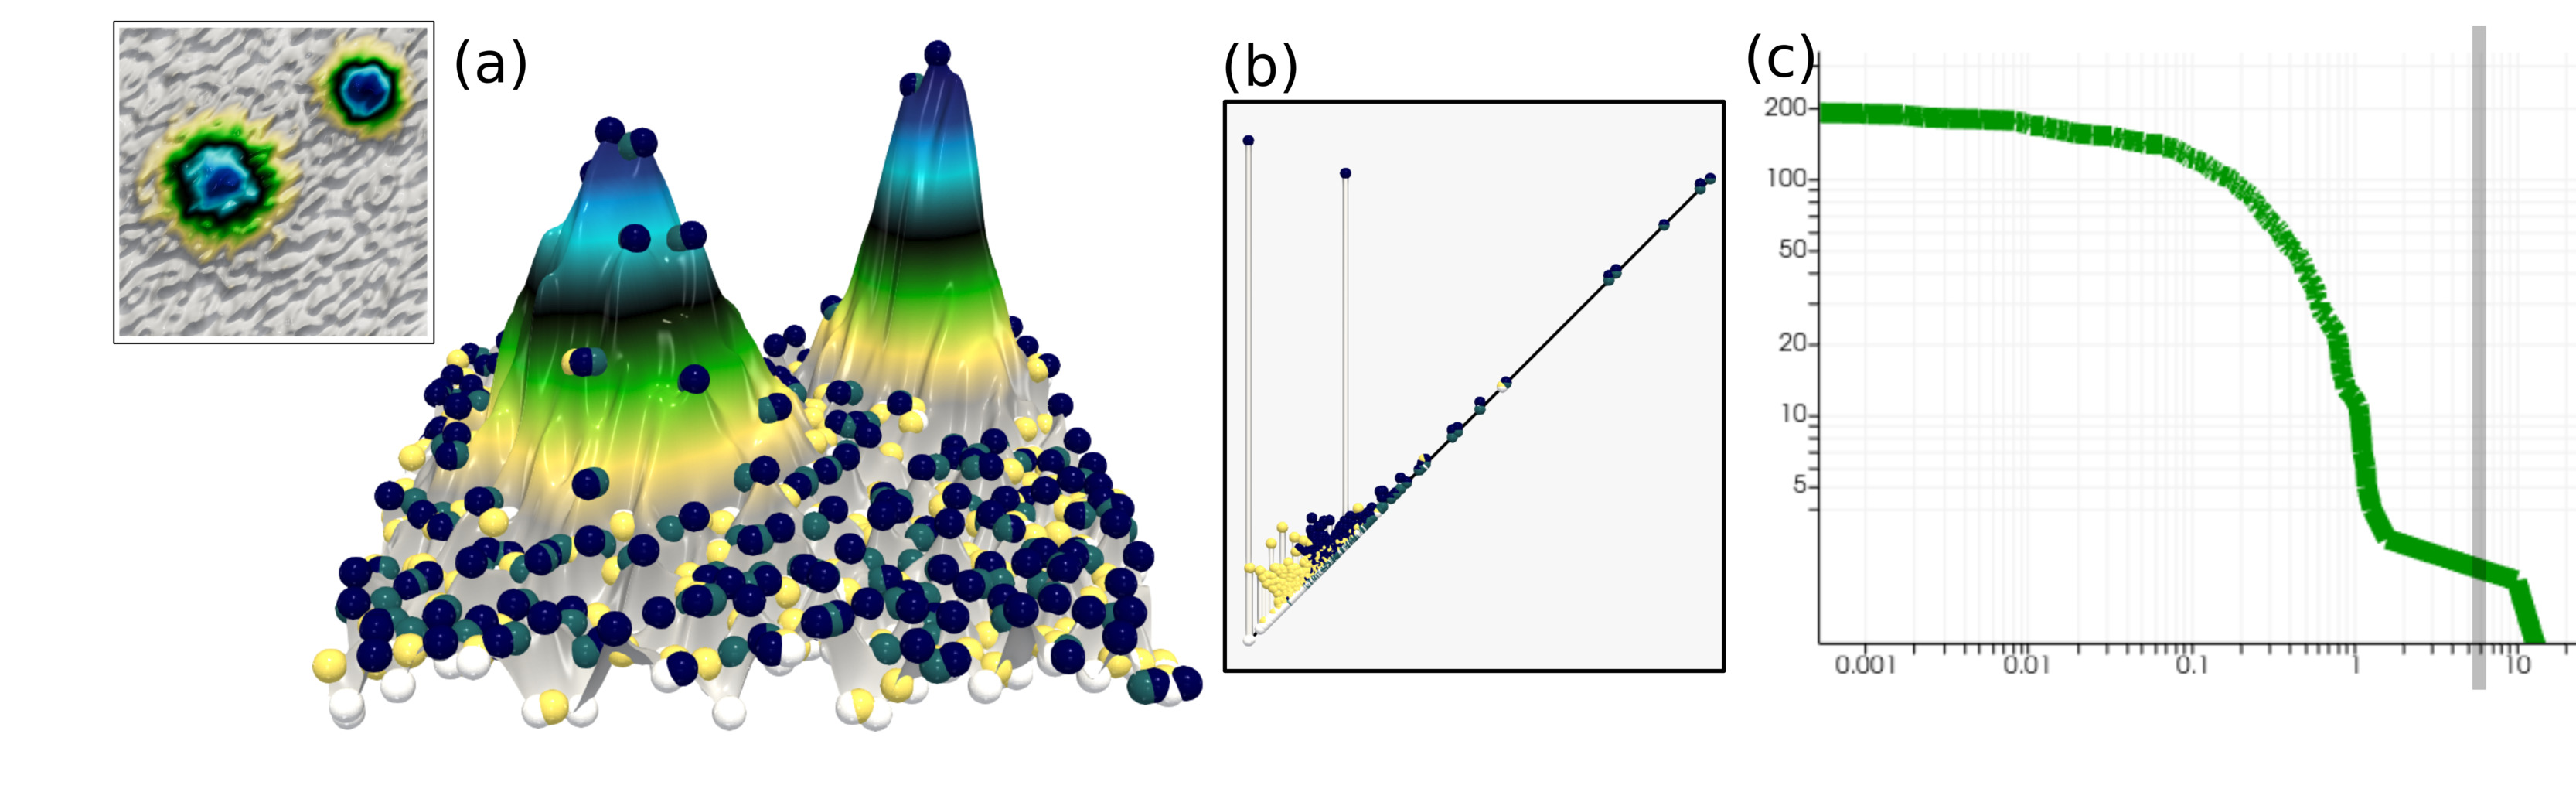
\includegraphics[width=\figureShrink\linewidth]{chapter4_topology_data_analysis/pictures/topo_gaussian.jpg}
 \caption{Critical points (spheres, white: minima, blue: maxima, other:
saddles), persistence diagram (b), persistence curve (c) of
a noisy (a) 2D
scalar field. The persistence diagram captures the main two hills of the
terrain as prominent persistence pairs (large vertical segments), while small
oscillations due to noise induce features near the diagonal.}
 \label{fig_toyTopology}
\end{figure}






\subsection{Topological data analysis}
\label{sec_topology}



This section presents the topological background of our work. It contains
definitions adapted from the Topology ToolKit \cite{ttk17}.
We refer the
reader to textbooks \cite{edelsbrunner09} for an introduction to
% computational
topology.

\noindent
\textbf{Input data.}
The input data is given as an ensemble of $N$ piecewise linear (PL) scalar
fields
$f_i : \domain \rightarrow \range$, with $i \in \{1, \dots,  N\}$, defined on a
PL 2-manifold $\domain$.
Specifically, $f_i$ represents the pointwise flow enstrophy
(\autoref{sec_simulation}) and $\domain$ is the Freudenthal triangulation
\cite{freudenthal42, kuhn60} of a $2$-dimensional regular grid, which is
periodic in both dimensions ($\domain$ is homeomorphic to a $2$-dimensional
torus). The triangulation is performed implicitly, by emulating the
simplicial structure upon traversal queries. Thus it induces no
memory overhead \cite{ttk17}.
The scalar values are given at the vertices of $\domain$ and are linearly
interpolated
on the simplices of higher dimensions.
$f$ is assumed to be injective on the vertices  of $\domain$.
This is
% easily
enforced in practice with a symbolic
perturbation inspired by Simulation of Simplicity \cite{edelsbrunner90}.


\noindent
\textbf{Critical points.}
Topological features in $f_i$ can be tracked with the notion of
\emph{sub-level set}, noted
$\sublevelset{{f_i}}(\isovalue)=\{p \in \domain~|
~f_i(p) < \isovalue\}$. It is defined as the pre-image of  $(-\infty,
\isovalue)$
by
$f_i$.
In particular, the topology of these sub-level sets (in 2D, their connected
components and cycles) can only change at special locations.
As $\isovalue$ continuously increases, the topology of
$\sublevelset{{f_i}}(\isovalue)$ changes at specific vertices of $\domain$,
called the \emph{critical points} of $f_i$ \cite{banchoff70}, defined next.
The \emph{star} of a vertex $v \in \domain$, noted $\Star(v)$,  is
the set of its co-faces:
$\Star(v) = \{ \simplex \in \domain ~|~ v < \sigma \}$.
It can be interpreted as the smallest combinatorial neighborhood around $v$.
The \emph{link} of $v$,
noted $\Link(v)$, is the set of the faces $\face$ of the simplices $\simplex$
of $\Star(v)$ with empty intersection with $v$:
$\Link(v) = \{ \face \in \domain ~ | ~ \face < \simplex, ~
\simplex\in \Star(v), ~ \face \cap v = \emptyset\}$.
The link of a vertex can
be interpreted as the boundary of its star.
The \emph{lower link} of $v$, noted $\lowerlink(v)$, is given by the
set of simplices of $\Link(v)$ which only contain vertices \emph{lower} than
$v$:
$\lowerlink(v) = \{ \simplex \in \Link(v) ~ | ~ \forall v' \in \sigma, ~ f_i(v')
< f_i(v)\}$. The upper link is defined symmetrically: $\upperlink(v) = \{
\simplex \in \Link(v) ~ | ~
\forall v' \in \sigma, ~ f_i(v') > f_i(v)\}$.
A vertex $v$ is \emph{regular}  if
and only if
both $\lowerlink(v)$ and $\upperlink(v)$ are simply connected. For
such vertices, the sub-level sets do not change their topology as they span
$\Star(v)$. Otherwise, $v$ is
a \emph{critical point}.
% of $f$ \cite{banchoff70}.
These can be classified with regard to their
\emph{index} $\Index(v)$.
It is equal to $0$ for local minima
($\lowerlink(v) = \emptyset$), to 2 for local maxima
($\upperlink(v) = \emptyset$) and otherwise to 1 for
saddles (\autoref{fig_toyTopology}a).
In practice, $f_i$ is enforced to contain only isolated, non-degenerate
critical points \cite{edelsbrunner90, edelsbrunner03}.
In the case of
the pointwise flow enstrophy, local maxima denote the center of vortices in the
turbulent flow. However, since the critical point characterization is based on a
classification which is only local (restricted to the link of each vertex), the
slightest oscillation in the data results in practice in the appearance of
spurious critical points, especially in the case of noisy data such as
turbulent flows. This motivates the introduction of an importance measure on
critical points, discussed next, in order to disambiguate vortices from noise.




\noindent
\textbf{Persistence diagrams.}
Several important
measures for critical points have been studied \cite{carr04},
including \emph{topological persistence} \cite{edelsbrunner02}, which is tightly
coupled to the notion of Persistence diagram \cite{edelsbrunner09}, which we
briefly describe here.
Persistence
assesses the importance of a critical point, based on the
lifetime of the topological feature it created (or destroyed) in
 $\sublevelset{{f_i}}(w)$, as one continuously increase the isovalue $w$.
In particular, as $w$ increases, new connected components of
$\sublevelset{{f_i}}(w)$ are created at the minima of $f_i$. The Elder rule
\cite{edelsbrunner09} indicates that if two connected
components, created at the minima $m_0$ and $m_1$ with $f_i(m_0) < f_i(m_1)$,
meet
at a given saddle $s$, the \emph{youngest} of the two components (the
one created at $m_1$) \emph{dies} in favor of the \emph{oldest} one (created at
$m_0$). In this case, a \emph{persistence pair} $(m_1, s)$ is created and
its
\emph{topological persistence} $p$ is given by $p(m_1, s) = f_i(s) - f_i(m_1)$.
All the local minima
can be
unambiguously
paired following this strategy, while the
global minimum is usually paired, by convention, with the global maximum.
The symmetric reasoning
can be applied to characterize, with saddle/maximum pairs, the life
time of the independent cycles of
$\sublevelset{{f_i}}(w)$.
Persistence pairs are usually
visualized with the \emph{Persistence diagram} $\diagram(f_i)$
\cite{edelsbrunner09}, which embeds each pair $(c, c')$, with $f_i(c) <
f_i(c')$,
as a point in the 2D plane, at location $\big(f_i(c), f_i(c')\big)$.
The  value $f_i(c)$ is 
% usually 
called the \emph{birth} of the
feature, while $f_i(c')$ is called its \emph{death}.
The
pair
persistence
can be
visualized as the height of the point to the diagonal.
Features with a high persistence stand out, away from the diagonal,
while noisy features are typically located in its vicinity 
(\autoref{fig_toyTopology}b).
The conciseness, stability \cite{edelsbrunner02} and expressiveness of this
diagram made it a popular tool
for data summarization tasks, as
it provides visual hints about the number, ranges and salience
of the features of interest.
To compare two datasets $f_i$ and $f_j$, persistence diagrams can be efficiently compared with the notion of $L_2$-Wasserstein distance \cite{CohenSteinerEH05,
Turner2014, Kerber2016} (we leave the practical study of distances between more
advanced topological descriptors  \cite{SridharamurthyM20,
pont_vis21} to future work). This distance is based on a bipartite assignment optimization problem (between the points of the two diagrams to compare), for which exact \cite{Munkres1957} and approximate \cite{Bertsekas81}
implementations are publicly available \cite{ttk17, ttk19}.
Specifically, we use in our approach the fast approximation scheme by Vidal et al. \cite{vidal_vis19}.
We refer the reader to \cite{Kerber2016, vidal_vis19, ttk19} for further
% practical
details.
Once the $L_2$-Wasserstein distance between two diagrams $\diagram(f_i)$ and $\diagram(f_j)$ is available (noted $\wasserstein{2}\big(\diagram(f_i), \diagram(f_j)\big)$), more advanced geometrical objects can be considered, such as \emph{Wasserstein barycenters} \cite{Turner2014, vidal_vis19}, which are
% representative
diagrams minimizing the sum of their distance to an ensemble of diagrams, and which consequently, can be considered as a reliable representative of the ensemble.
This notion of \emph{barycenter}
% it
is conducive to the design of clustering algorithms.
% , directly in
% the Wasserstein metric space.
% In particular,
The $k$-means algorithm
% \cite{elkan03, celebi13}
can be easily extended,
by using $\wasserstein{2}$ to measure distances between diagrams, and by
considering as cluster centroid, at each iteration of the $k$-means, the
 barycenter of the cluster.


\noindent
\textbf{Persistence curves.}
A popular, alternate, representation of persistence features is the notion of
\emph{Persistence Curve}, noted $\persistentCurve(f_i)$, which plots the
population of persistent pairs as a function of their persistence.
Specifically, it encodes the number of pairs (Y axis) whose persistence is
\emph{larger} than a threshold $\epsilon$ (X axis).
For $X=0$, $Y$ is equal to the total number of persistence pairs, while for the
largest values of $X$, $Y$ indicates the number of prominent, high-persistence
features (\autoref{fig_toyTopology}c).
In practice, large
plateaus in this curve will indicate \emph{stable} persistence ranges, for
which no (or few) topological features are present in the data. These 
correspond to \emph{separations} (vertical line, \autoref{fig_toyTopology}c) 
between populations of topological
features of distinct persistence scales, typically the noise (low $X$
values) and the persistent features (high $X$ values).


\section{Case Study}

\label{sec_caseStudy}
In this section, we give \emph{(i)} a description of the ensemble (made publicly
available \cite{data})
% data
representing the Kelvin Helmholtz Instabilities (KHI) computed on 
%the CEA 
our institution's
facilities.
% which has 
% been 
% .
Next, we state \emph{(ii)} the challenges in understanding
such phenomena and we
% edict
provide
\emph{(iii)} theoretical hypothesis that our
experimental protocols have to verify.   

\begin{figure}
 \centering
 \vspace{-1ex}
 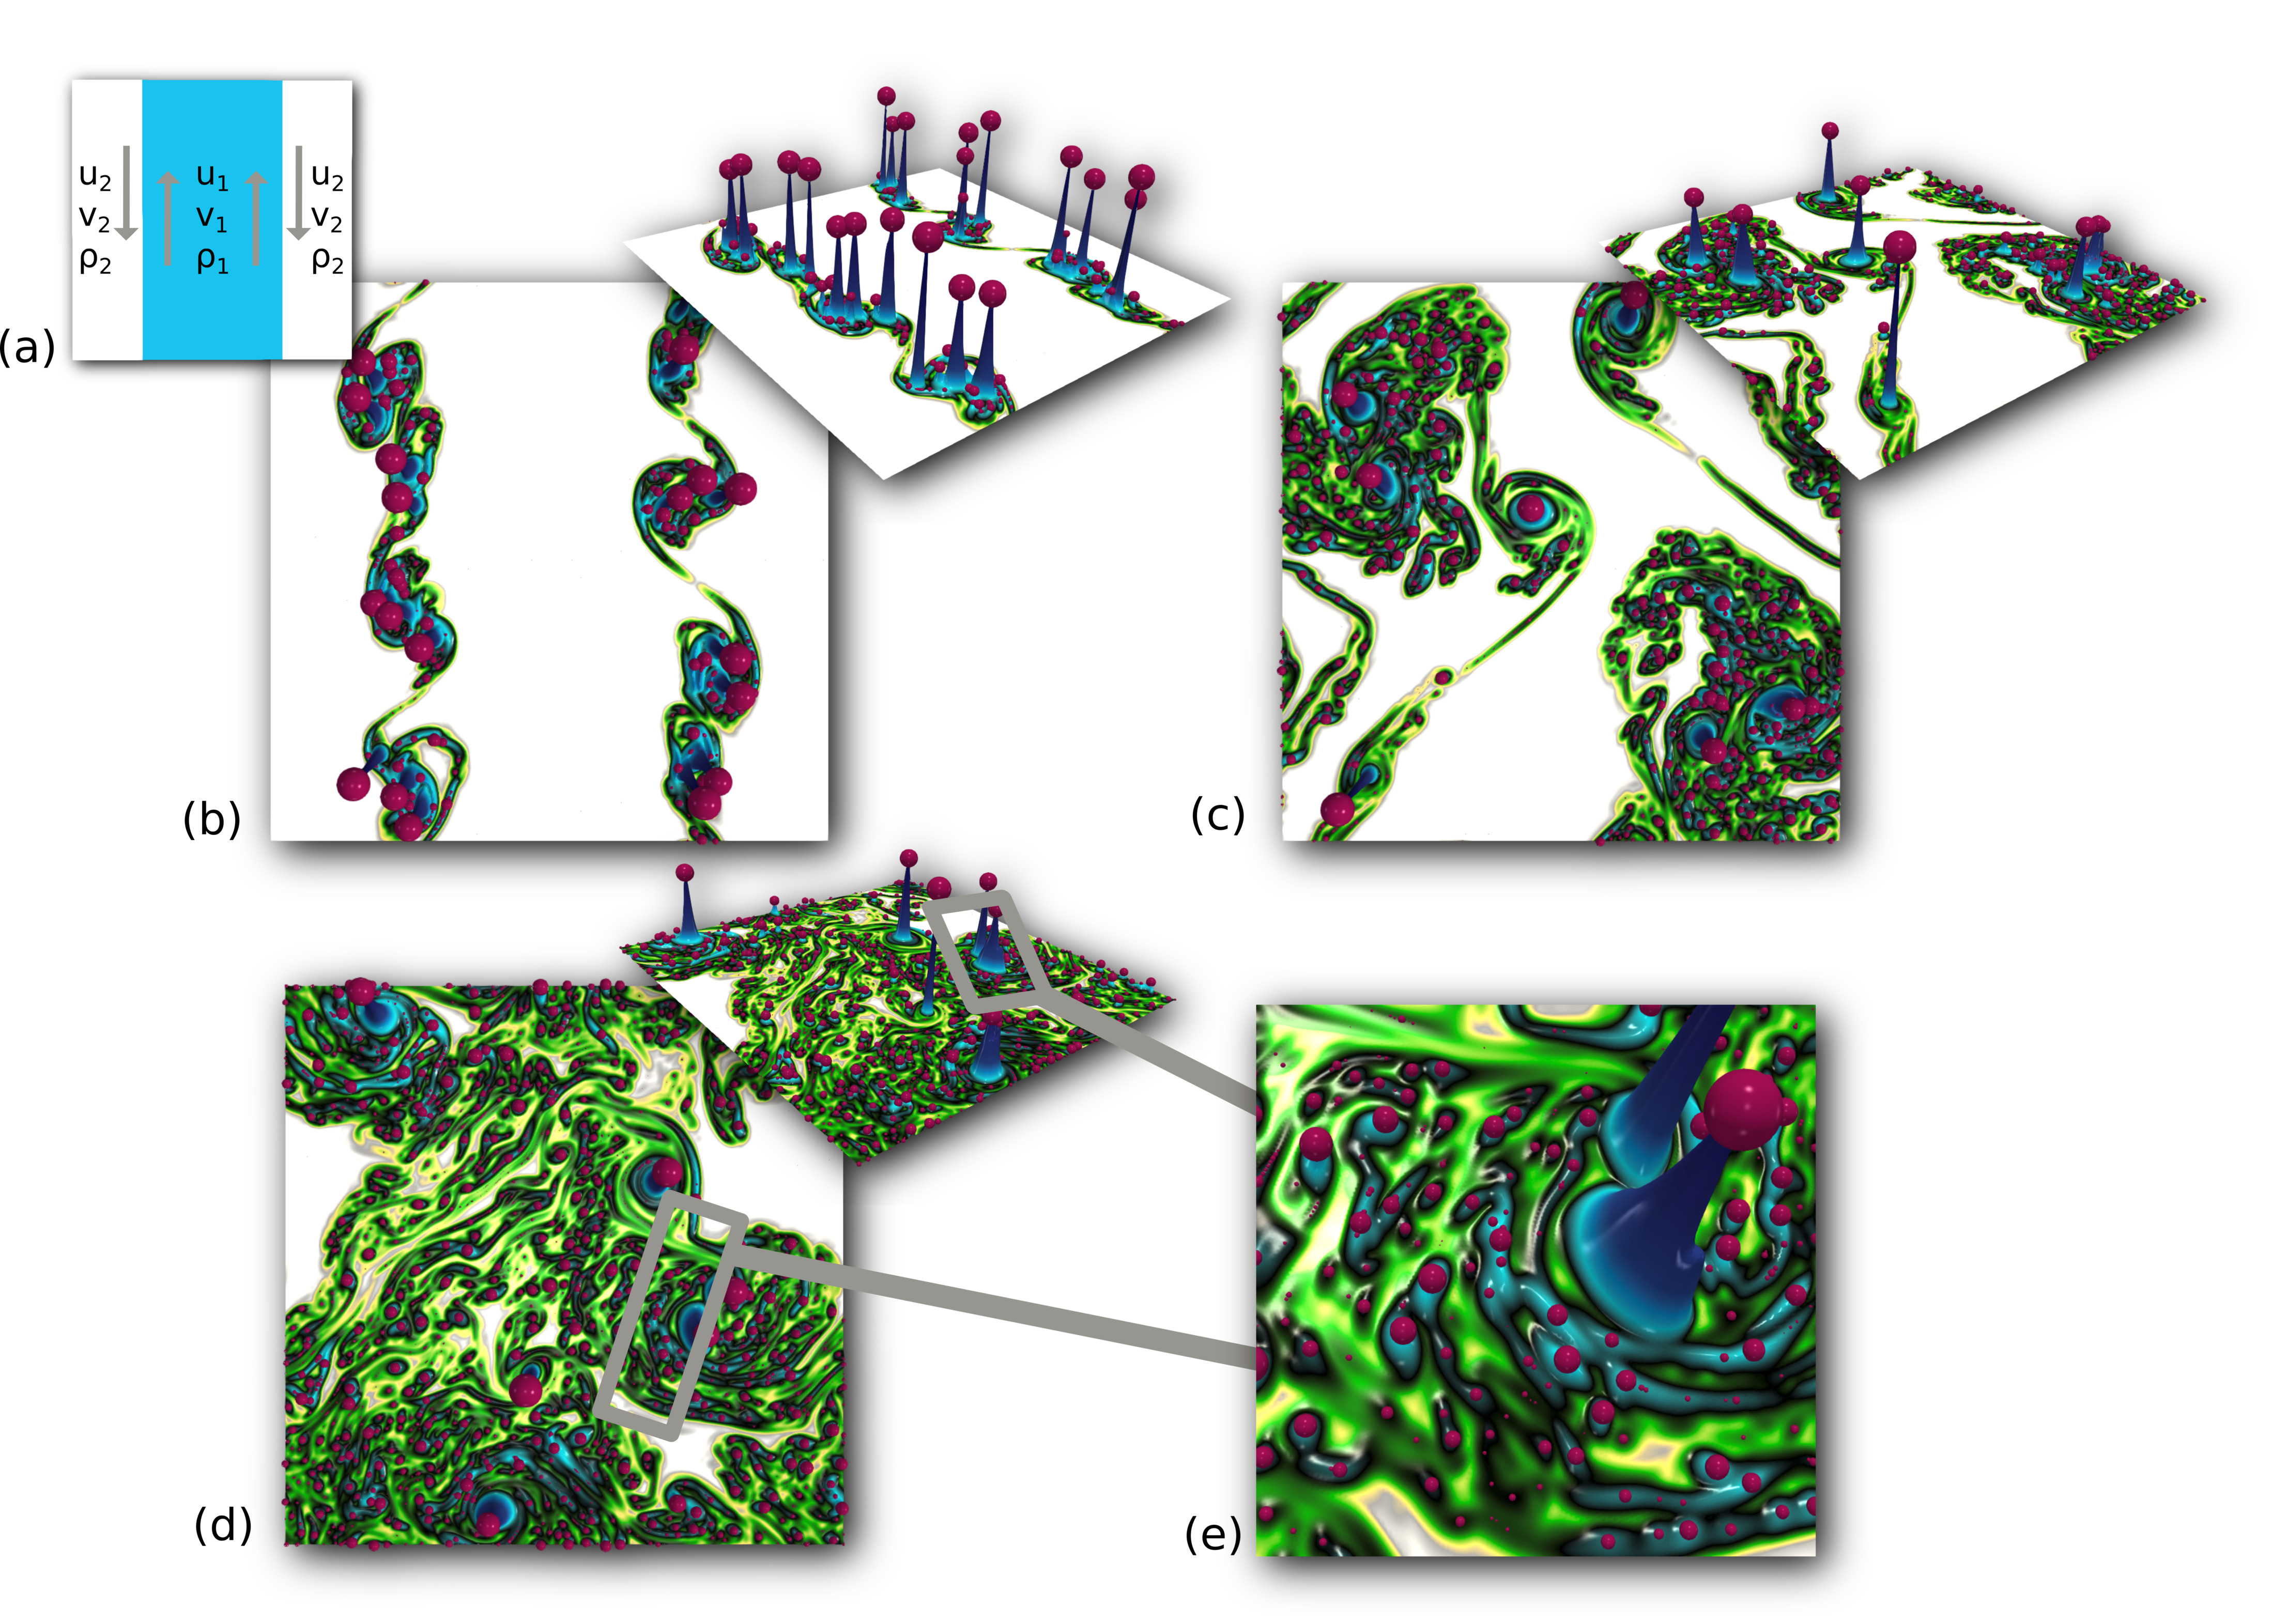
\includegraphics[width=\figureShrink\linewidth]{chapter4_topology_data_analysis/pictures/init_case.jpg}
 \vspace{-2ex}
 \mycaption{Initialization of the Kelvin-Helmholtz instability (a). This simulation was obtained
with the AUSM$^+$-UP solver with a TENO 5 order interpolation at physical times $0.25$(b), 
$0.75$(c) and $1.25$(d). Red spheres scaled by the persistence represent the maximum critical points. Zoom of the turbulence structures (e).}
  \vspace{2ex}
 \label{initcase}
\end{figure}

\subsection{Data description}
The initialization of the KHI was generated with two fluids of different 
densities ($\rho_{1}$, $\rho_{2}$) (\autoref{initcase}a). The
different velocities of opposite direction ($\{u _{1},v_{1}\},\{u _{2},v_{2}\}$) 
of the fluids create a shearing zone where the turbulence appears with the KHI 
(\autoref{initcase}b). While the instability develops over time the main 
vortices grow (\autoref{initcase}c). After a longer simulation time, the main 
structures keep evolving (\autoref{initcase}d) and a large number of 
small-scale vortices appear in the vicinity of large-scale vortices
% around the main structures 
(\autoref{initcase}e) 
leading to a complex turbulent flow. This variation in vortex scale,
% of the
% vortices,
in addition to the chaotic flow geometry,
% of the flow,
is notoriously
challenging for the analysis of turbulent flows.

\begin{table}
\centering
\scalebox{0.8}{
\begin{tabular}{|c|c|c|c|c|c|c|}
\hline
Parameter            & Resolution           & Order                &  Time       
       &  Solver              &  Scheme              &  Total              \\ 
\hline
\hline
                     &                      &                      &             
         &  HLL            &                 &                \\
                     &  256                 &      5               &       t$_0$ 
         &  SLAU2          &  TENO         &                \\
Value                &  512                 &      7               &       t$_1$ 
         &  AUSM$^+$-UP         &  WENO-Z        &                \\
                     &  1024                &                      &       t$_2$ 
         &  Roe            &                &                \\
                     &                      &                      &             
         &  HLLC           &                &                \\                  
                                             
\hline
\hline
Number&3&2&3&5&2&180\\
\hline
\multicolumn{1}{l}{} & \multicolumn{1}{l}{} & \multicolumn{1}{l}{} & 
\multicolumn{1}{l}{} & \multicolumn{1}{l}{} & \multicolumn{1}{l}{} & 
\multicolumn{1}{l}{} 
\end{tabular}
}

\caption{Parameter space of the HYPERION simulation code leading to a total of 180 members for the ensemble dataset used in this study.}
\vspace{-3ex}
\label{tab_parameters}
\end{table}

% This is why, in the section 
% \autoref{sec_experimentalResults} we study how the topological analysis of the 
% % enstrophy can capture features in the KHI and thus help us to compare them. 

The HYPERION simulation code introduced in \autoref{sec_simulation} has been 
used to generate the ensemble dataset. All the simulations have been run on a 
supercomputer 
% of the CEA 
at our institution. Each simulation have been executed in parallel using 16 MPI processes and have been distributed over the supercomputer. The total 
simulation took about 745 CPU hours. The raw data has been dump on disk with the 
metadata stored in XDMF files and the scalar fields in HDF5 files leading to 14 
GB for the entire ensemble dataset. We processed these results to extract the 
enstrophy scalar field (\autoref{eq:enstrophy}) and stored it to a VTK file 
format \cite{Kitware:2003} using an image data structure for regular grids 
(VTI). This reduces the entire ensemble to 600 MB. 

The ensemble dataset corresponds to different computational configurations for 
the same turbulent instability. HYPERION handles different parameter types such 
as scalars or enumerations, which allows the users to compute various numerical 
simulations in the same parametric study. The resolution of the 2D regular grid, 
the simulation time, the interpolation scheme, the order of interpolation and 
the Riemann solvers presented in \autoref{sec_background} are our different 
parameters. \autoref{tab_parameters} details the parameter types and values as 
well as the number of samples per parameter, leading overall to an ensemble of 
$3\times2\times3\times5\times2=180$ members illustrated \autoref{fig_teaser}a. 
Each parameter value of \autoref{tab_parameters} used to run the simulation has 
been stored as meta-data in the VTI files (i.e. \emph{Field Data} in the VTK 
terminology)  to keep track of the computational configuration for later 
analysis down the pipeline.
In order to ease the exploration of the ensemble dataset, we defined a 
SQL-type database using the cinema database feature of TTK \cite{ttk17, ttk19}. 
This representation facilitates the extraction of sub-samples of the ensemble, 
based on standard SQL queries on the simulation parameters 
(\autoref{tab_parameters}).

% This database eases the query to extract sub-samples of the ensemble using the 
% input parameters referenced in \autoref{tab_parameters}.\julien{référencer 
% l'annexe pour le détail technique des temps ?}



\begin{figure}
 \centering
 \vspace{-1ex}
 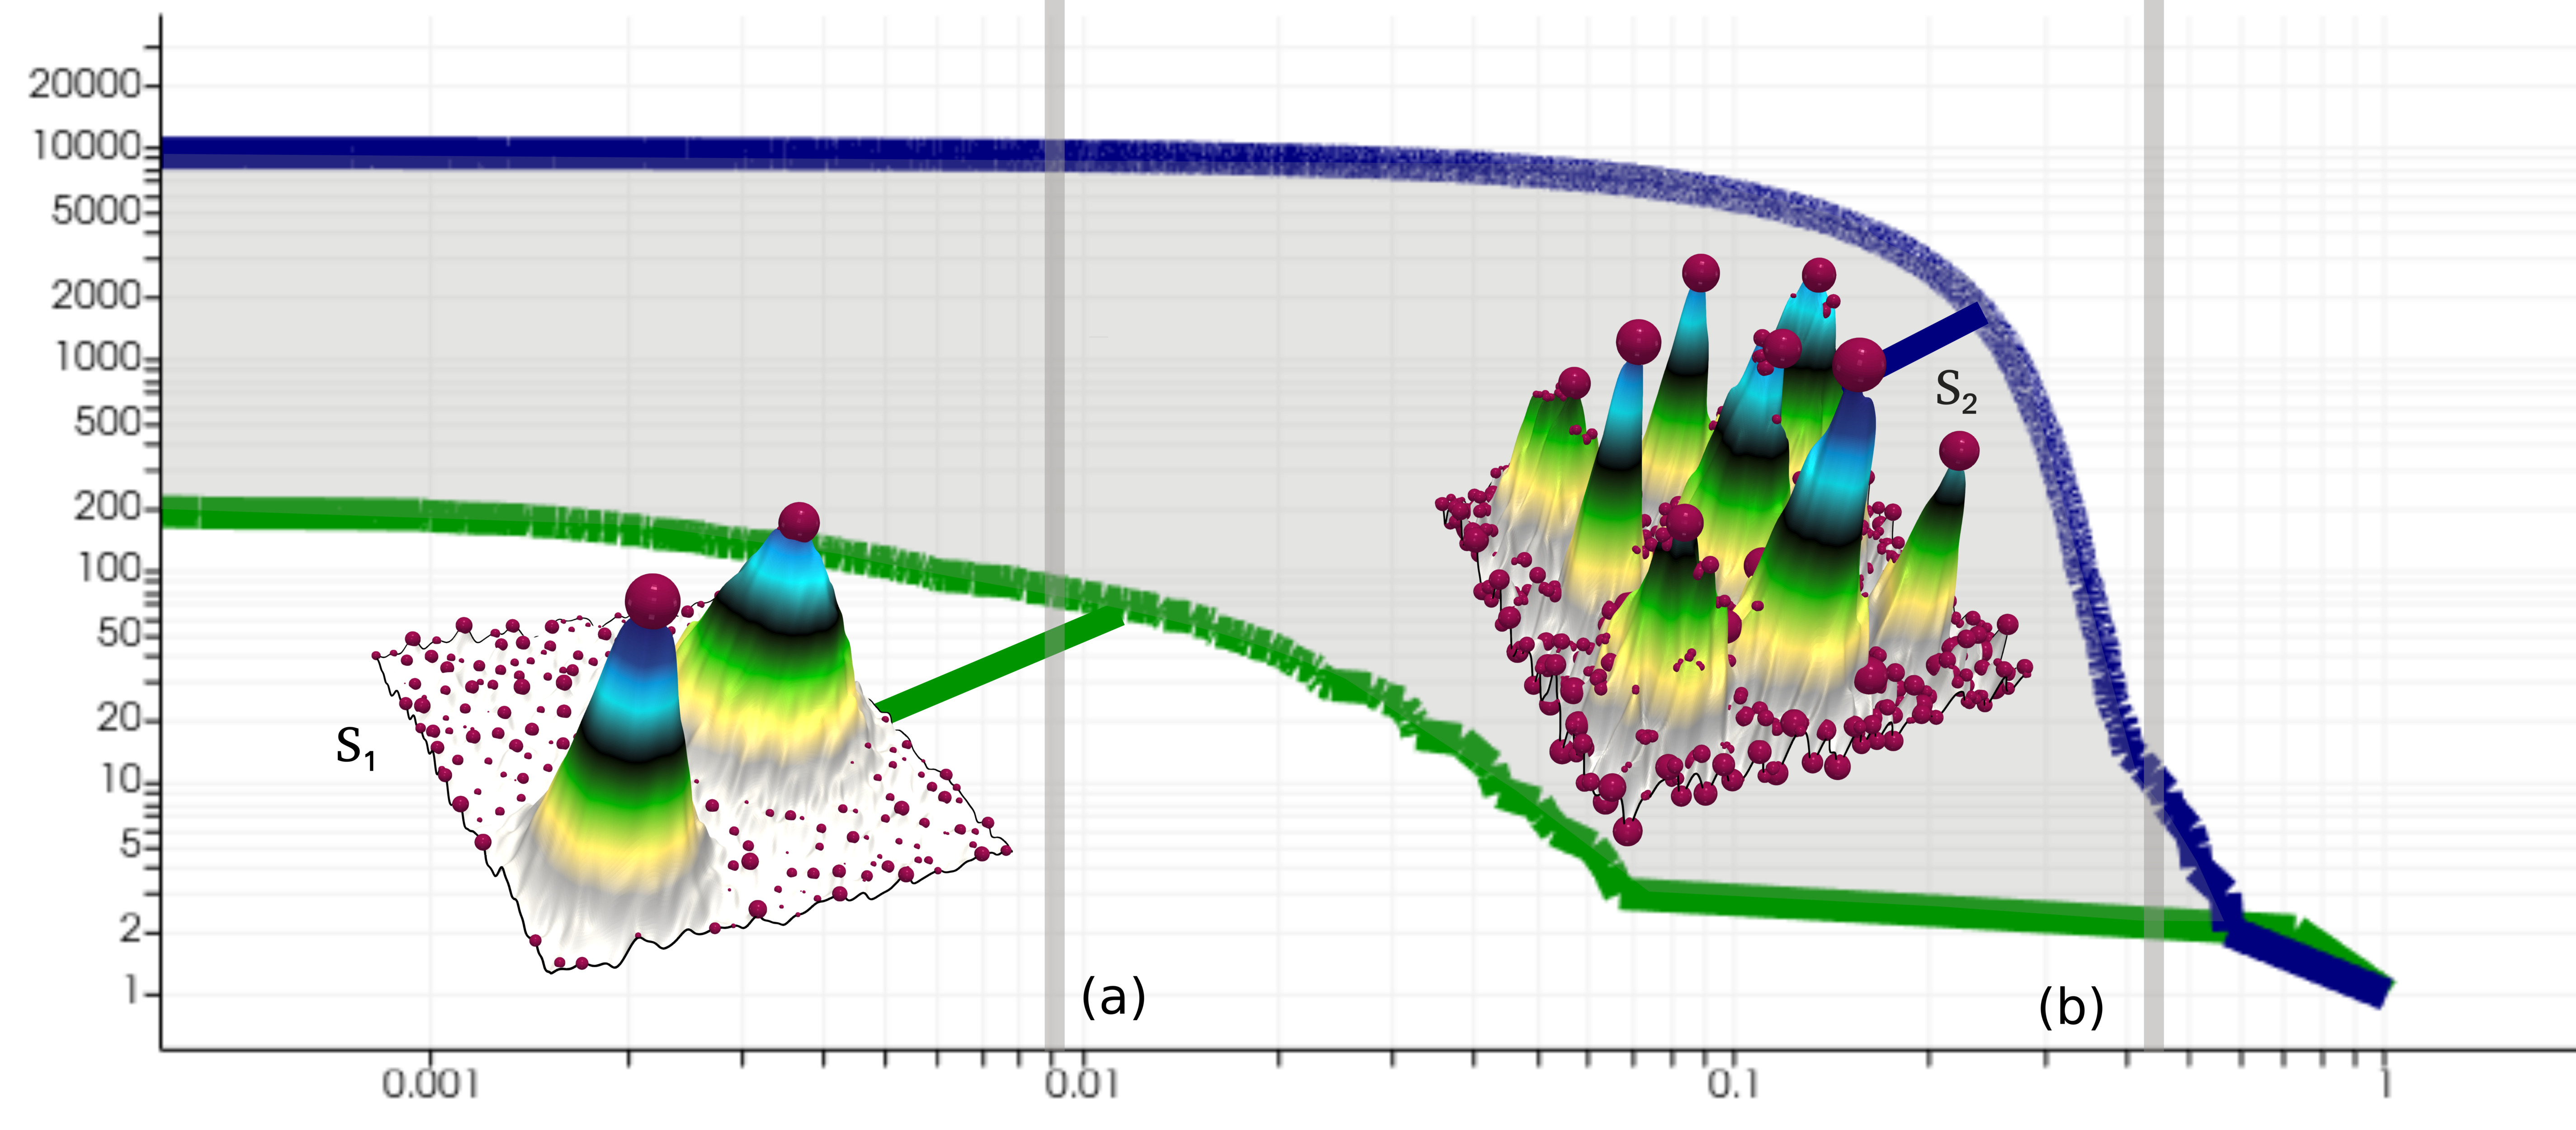
\includegraphics[width=\figureShrink\linewidth]{chapter4_topology_data_analysis/pictures/gaussian_courbe.jpg}
 \mycaption{Persistence curves for two input scalar fields (X-axis: persistence threshold, Y-axis: number of maxima more persistent than X). $S_1$ generated with two Gaussian functions with noise and $S_2$ with 10 Gaussian functions with a stronger noise. Maxima critical points are represented by red spheres scaled by persistence. Vertical line corresponds to
 (a) small persistence critical points, (b) to high persistence. The grey area is the integral difference between the two curves.}
 \label{fig_gaussian_curve}
\end{figure}

\subsection{Problem statement}

% For numerical computation in fluid dynamics there are several methods of interpolation and Riemann solvers.
% For today's engineers who design vehicles it is important to use accurate methods to recover for example heat fluxes, pressure at the walls to be able to dimension correctly their future vehicles.
% Nevertheless, it is also necessary to take into account the calculation time which can be extremely high, especially with 3-dimensional calculations.
% The calculation of the turbulence is then important because this phenomenon will bring fluctuations of the data that we analyze and it is then necessary to capture it with precisions too.
% It is a fractal phenomenon that we analyze by averaging on the domain a value to look at scpectra later.
% With this traditional treatment it is difficult to see a real difference between the numerical methods and especially for the solvers.
% That's why we want to use the topology to maybe guide our choice of numerical methods.
% -- 
Vehicle design, be it in an automotive or aeronautical context, is well known for its high number of constraints that are nowadays most often handled with the help of computational techniques.
In the aeronautical world for instance, engineers today face an incredible challenge wherein they have to be able to predict, at the same time, integral quantities at the wall of the vehicle such as heat flux or pressure as well as three-dimensional phenomena such as flow discontinuities and turbulence.
In other words, engineers have to deal with multiple types of physics and phenomena that have markedly different length- and time-scales but whose interactions are still of great importance to the accuracy of their predictions.
With limited time and resources to conduct the computer-aided simulations, the traditional approach is to rely on numerical strategies that temporally average most of the three-dimensional phenomena and rely more or less on models of turbulence to yield a fast and reasonable forecast.

Even in such a context of approximate simulations, the choice of the ingredients of the numerical recipe matters - methods of reconstruction, Riemann solvers, etc.
Making the right choices can indeed bring a significant increase in fidelity to the engineer, especially in terms of turbulence, by lessening the need for modeling and henceforth bring more margin in the design of the vehicle.
Turbulence is however by nature a chaotic phenomenon and conducting a systematical study of the impact of the different
% aforementioned
numerical ingredients thereupon might prove tricky for a simple reason: beyond a certain level of accuracy, everything will \emph{look} the same.
Detecting the benefits of one method compared to another in that situation will be next to impossible - that is, with traditional techniques.
We propose here to use the ability of topological analysis to discern features that stay otherwise hidden in traditional fluid dynamics postprocessing to help with the choice of the right numerical ingredients. 



\subsection{CFD Hypotheses}
\label{sec_hypotheses}
This section introduces the hypotheses provided by CFD experts, documenting their expectations about ensemble flow variability.
% in the ensemble.}

% \florent{Here are the assumptions considered in this study, provided by CFD experts, with a literature search.}

\label{Hypotheses}
\noindent
\textbf{Hypothesis H1.}
% It is assumed that
TENO induces more turbulence (i.e. more critical points) than
% the
WENO-Z, for all configurations.\\
% no matter the resolution, the time or the solver is.\\
\textbf{Hypothesis H2.}
Order 5 and 7 are equivalent for Kelvin Helmholtz instabilities.\\
% In the literature, studies have been conducted on turbulence and notably on Kelvin Helmholtz to show that orders 5 and 7 are equivalent. We therefore try to find an independence of the orders using our topological analysis.\\
\textbf{Hypothesis H3.}
The HLL solver should provide a significantly distinct description, for all configurations.\\
% It is assumed that the HLL solver describes very differently the instabilities for all resolutions and schemes. It's a dissipative solver and doesn't take into account the dissipative
% contact discontinuities.\\
\textbf{Hypothesis H4.}
The HLLC and Roe solvers should provide equivalent outputs for all configurations.\\
% (and should therefore belong to the same cluster).\\
% It is assumed that HLLC and Roe are in the same cluster for all resolutions and schemes. These solvers are of FDS type, they take into account the contact discontinuities, but do not adapt to all Mach.\\
\textbf{Hypothesis H5.}
The
% It is assumed that
SLAU2 and AUSM$^+$-UP solvers should provide equivalent outputs for all configurations.\\
% are in the same cluster for all resolutions and schemes.
% They are FTS type solvers, they have the characteristics of being not very dissipative and they adapt to all speeds.\\

The above hypotheses are direct consequences of
% prior experimental
observations, or
% solver
design choices. For instance, the TENO scheme has been reported to capture turbulence more accurately \cite{peng2021efficient}, which is expressed by Hypothesis H1. Similar kinetic energy curves (\autoref{energie}) have been reported for the orders 5 and 7, which is expressed by Hypothesis H2. The HLL solver, which is a dissipative approach, is known to model contact discontinuities poorly in contrast to more recent solvers, which is expressed in Hypothesis H3 \cite{toro2013riemann}. Finally, unlike the SLAU2 and AUSMUP (FTS type) solvers, the HLLC and RoE (FDS type) solvers have been reported to provide unphysical results at both low and high velocities (resulting in local oscillations in pressure and density), which is expressed in Hypotheses H4 and H5. %\cite{qu2021review}.

From a practical point of view, the validation of these hypotheses has a major impact for the engineers when setting up their simulations. For instance, the validation of the Hypothesis H1 would justify the usage of a more computationally expensive scheme (TENO), while the validation of the Hypothesis H2 would enable the usage of less computationally expensive orders (5 instead of 7). Finally, the validation of the Hypotheses H3, H4, and H5 would help engineers properly select the most appropriate solvers, based on their flow characteristics.
% expected velocities.
Then, overall, the validation of these hypotheses
% is important towards the
would provide reliable rules-of-thumb for the tuning of the solvers,
% enables more confidence when
% proper
% tuning of the solvers,
to achieve the best balance between accuracy and speed.

% \florent{Referring to the publication of liu fu,(Add ref \cite{peng2021efficient}) who developed the TENO scheme, and who compared it to the weno scheme on several test cases, the TENO has the ability to capture with more accuracy the turbulence phenomenon.  By looking at the topological approaches to the results obtained between these two schemes we should observe differences in the number of structures that are reconstructed(H1).}
% \florent{A study on weno(ref) schemes, using a KHI as a test case, shows that for order 5 and 7, a similar result is obtained on the kinetic energy curves (\autoref{energie}).}
% \florent{Assumptions H4 and H5 allow us to compare Riemann solvers that do or do not calculate all velocities in a numerical simulation. According to the literature (add ref). The HLLC and ROE solvers fail to calculate both high and low velocities, which leads to small oscillations (pressure or density) in the simulation results, unlike the SLAU2 and AUSMUP solvers.
% Validating the Hypotheses will help engineers to choose which tools to use to set up their numerical simulations by minimising the computational cost and to gain precision in the numerical methods used.}




\subsection{Baseline analysis}
Traditional approaches for turbulent data analysis (\autoref{energie}) are based on an average of
quantities of interest, such as flow energy (\autoref{sec_relatedWork}).
The $L_2$ norm is another established distance for comparing scalar fields. Both strategies bear similarities in their averaging artifacts: they cannot distinguish the contribution
of small structures from the global flow, because these are masked by the weight
of larger vortices.
%
% However, this average strategy
% % the energy or the enstrophy (see
% % \autoref{sec_relatedWork} and \autoref{energie}).
% such an averaging is similar to the averaging
% effect of the $L_2$-norm, when used for comparing enstrophy fields.
% % These averages correspond to the calculation of $L_2$-distances between the
% % solutions.
% In particular, this distance does not allow to see the contribution
% of the small structures to the global flow because they are masked by the weight
% of larger structures.
Moreover, the $L_2$-norm is also very sensitive to mild geometric variations,
whereas the chaotic nature of turbulent flows induces major geometric
variations between ensemble members.
This motivates the usage of  topological methods to capture
features in the KHI that will help us compare the members
(\autoref{sec_experimentalResults}). In the remainder, we will systematically compare our protocols based on topological distances (\autoref{sec_protocols}) to the $L_2$ norm, considered as the baseline approach, and detailed comparisons will be provided (\autoref{sec_experimentalResults}).




\section{Evaluation protocols}
\label{sec_protocols}
In this section, we present 3 protocols which can be used to verify the
hypotheses detailed in \autoref{Hypotheses}. One can directly use these
algorithms on the ensemble dataset. It corresponds to $(i)$ the separation of
the schemes and the independence of the orders, $(ii)$ the unique behavior of
the HLL solver and $(iii)$ similarities in class of solvers.


\subsection{Persistence curves}
\label{sec_persistence}
With this protocol (illustrated on toy examples, \autoref{fig_gaussian_curve}), we want to validate hypothesis H1 (\autoref{Hypotheses}) to discriminate the interpolation schemes TENO and WENO-Z regarding the differences in the enstrophy field. With this protocol, we also want to validate hypothesis H2 (\autoref{Hypotheses}) to confirm the independence of the orders \cite{san2015evaluation}. To better characterize the vortices influencing the turbulence, we use persistence curves (\autoref{sec_topology}). These curves will
allow us to threshold the structures (the eddies) at different scales and
thus to easily compare the number of small (\autoref{fig_gaussian_curve}a) and large (\autoref{fig_gaussian_curve}b) eddies using the integral of the persistence curve.

For the differentiation of the schemes, we take 5 simulation configurations where the physical time ($t_0,t_1,t_2$), the resolution ($256\times 256$, $512\times 512$, $ 1024\times 1024$) and the order (5,7) are fixed per sample (\autoref{tab_parameters}). The variation is the interpolation scheme (TENO, WENO-Z). For the order independence, 5 configurations are also chosen by fixing the physical time ($t_0,t_1,t_2$), the resolution ($256\times 256$, $512\times 512$, $ 1024\times 1024$), the scheme (TENO or WENO-Z). The variation is done on the order (5,7). Besides different input variations,
% to build the configurations,
this protocol is the same for testing H1 and H2.

The persistence curves are generated for all the samples. Then, we average the 5 persistence curves (one per solver) to obtain 2 average persistence curves with respect to the variable parameters (schemes or orders). Finally, we compute the difference of the integrals between the two averaged curves (grey area on \autoref{fig_gaussian_curve}). The small values on the curves under a persistence of $10^{-6}$ correspond to numerical noise coming from the different simulation steps. They are removed from the computation of the integral with a threshold at $10^{-6}$(\autoref{fig_gaussian_curve}.a). The integral curve difference corresponds to our metric allowing to precisely describe the similarity in the topology of the critical points. Bigger is the integral, the more different the topology of the flow is. Thus, to verify hypothesis H1 related to the scheme, we want the difference of the integrals to be high. To verify hypothesis H2 related to the orders, we want the difference of the integrals to be close to zero.


\begin{figure}
 \centering
 \vspace{-1ex}
 
\includegraphics[width=\figureShrink\linewidth]{chapter4_topology_data_analysis/pictures/gaussian_distance_to_the_rest.jpg}
 \mycaption{
 Wasserstein distance matrix for five inputs $S_1$, $S_2$, $S_3$,$S_4$, $S_5$
 generated respectively with two, five, four and three Gaussians
%  functions
 with varying noise.
% different noise levels.
The sum of each
matrix line
% line of the matrix
is
% computed and
normalized with respect to the scalar-field that maximizes the distances, here
$S_1$. We see that $S_1$ with only two Gaussians is very far from the other
datasets.}
 \label{gaussian_distance}
\end{figure}
\begin{figure}
\vspace{-1ex}
 \centering % avoid the use of \begin{center}...\end{center} and use \centering
 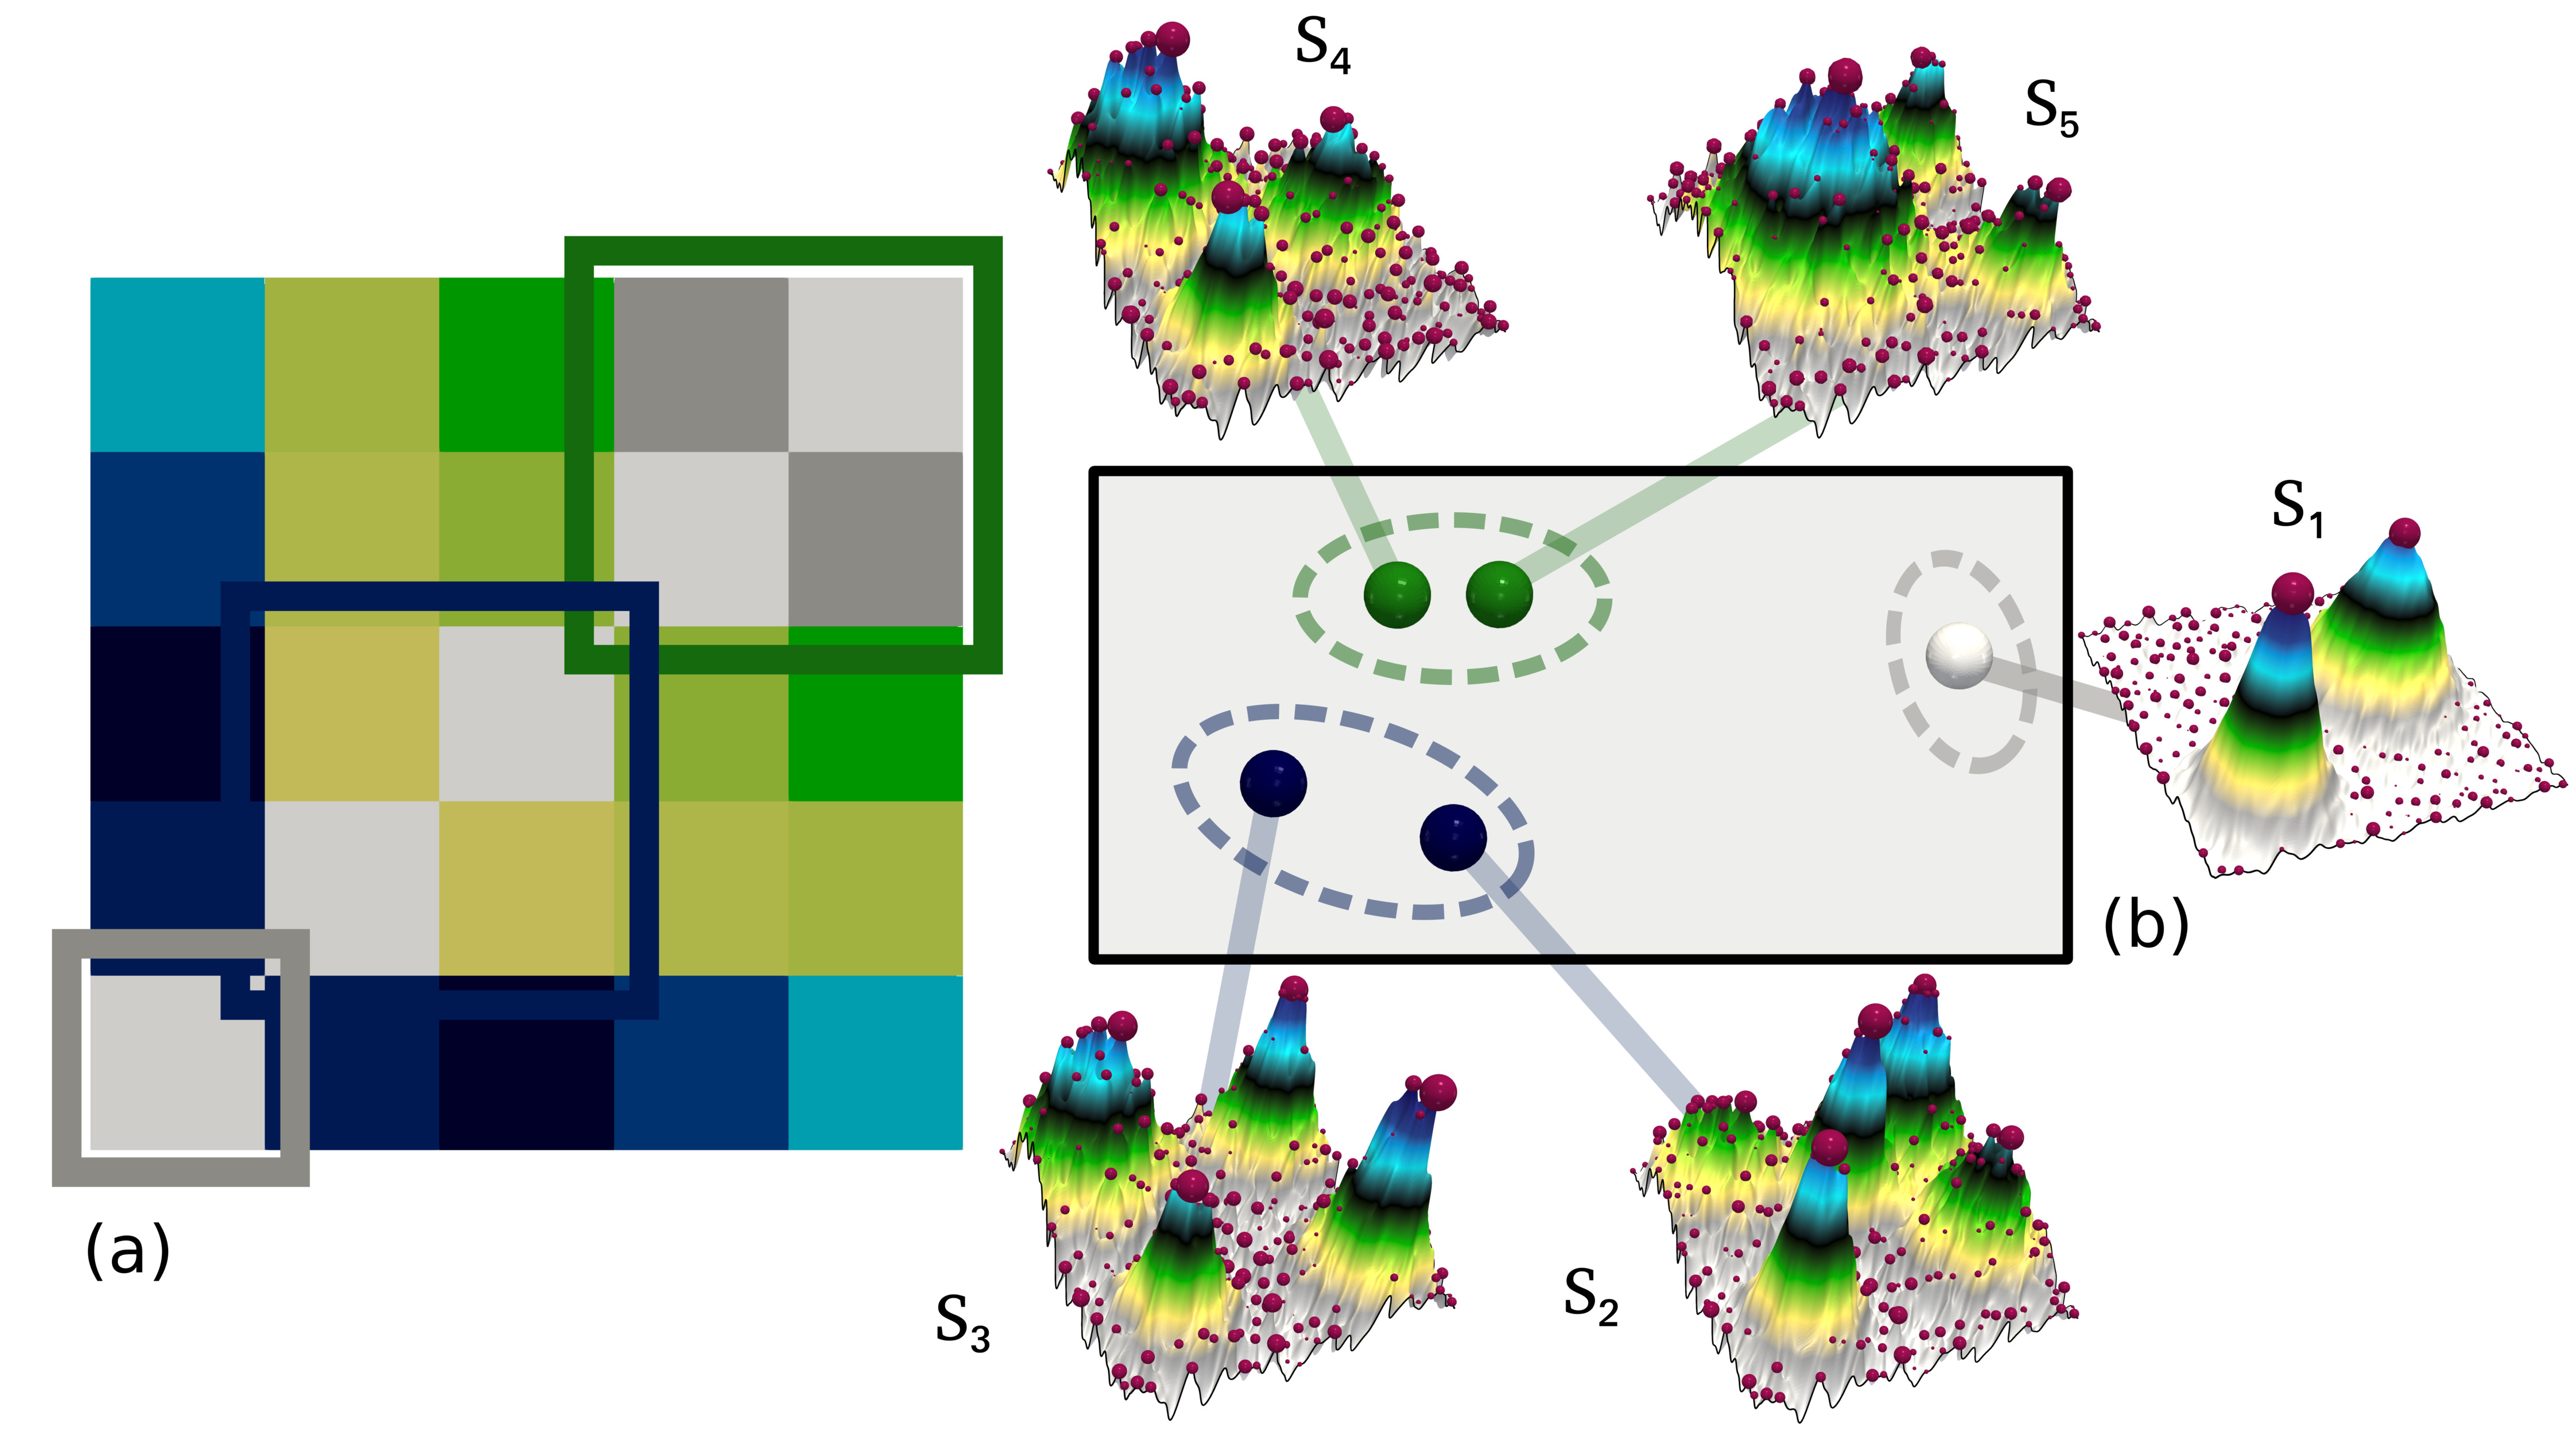
\includegraphics[width=\figureShrink\linewidth]{chapter4_topology_data_analysis/pictures/gaussian_cluster.jpg}
 \mycaption{
 Wasserstein distance matrix for five inputs $S_1$, $S_2$, $S_3$, $S_4$, $S_5$ generated respectively with two, five, for and three Gaussian
functions with different noise levels. Point cloud of the inputs in the Wasserstein distance space colored according to the clusters obtained with the k-means clustering method. We can see that each terrain in a cluster has the same number of Gaussian and level of noise.}
 \label{gaussian_cluster}
\end{figure}
\begin{figure*}
 \centering % avoid the use of \begin{center}...\end{center} and use \centering
 
\includegraphics[width=\figureShrink\linewidth]{chapter4_topology_data_analysis/pictures/KHI_courbes.jpg}
 \mycaption{
Schemes (left) and order (right) studies.
% , left orders study.
Average
persistence curves for 5 configurations with variations of : a (WENO-Z,5), c
(WENO-Z, 7), f (WENO-Z, 5), h (TENO,5). (b,g) persistence curves at $t_0$ (top),
$t_1$ (middle), $t_2$ (bottom).
 Vertical lines on the curves correspond to critical points of small (left) and
high (right) persistence.
% critical points (left) and high persistence (right).
(d,e) Integral differences (grey area) between average persistence curves for
all variations.}
\vspace{2ex}
 \label{curv}
\end{figure*}

\begin{figure*}
 \centering
 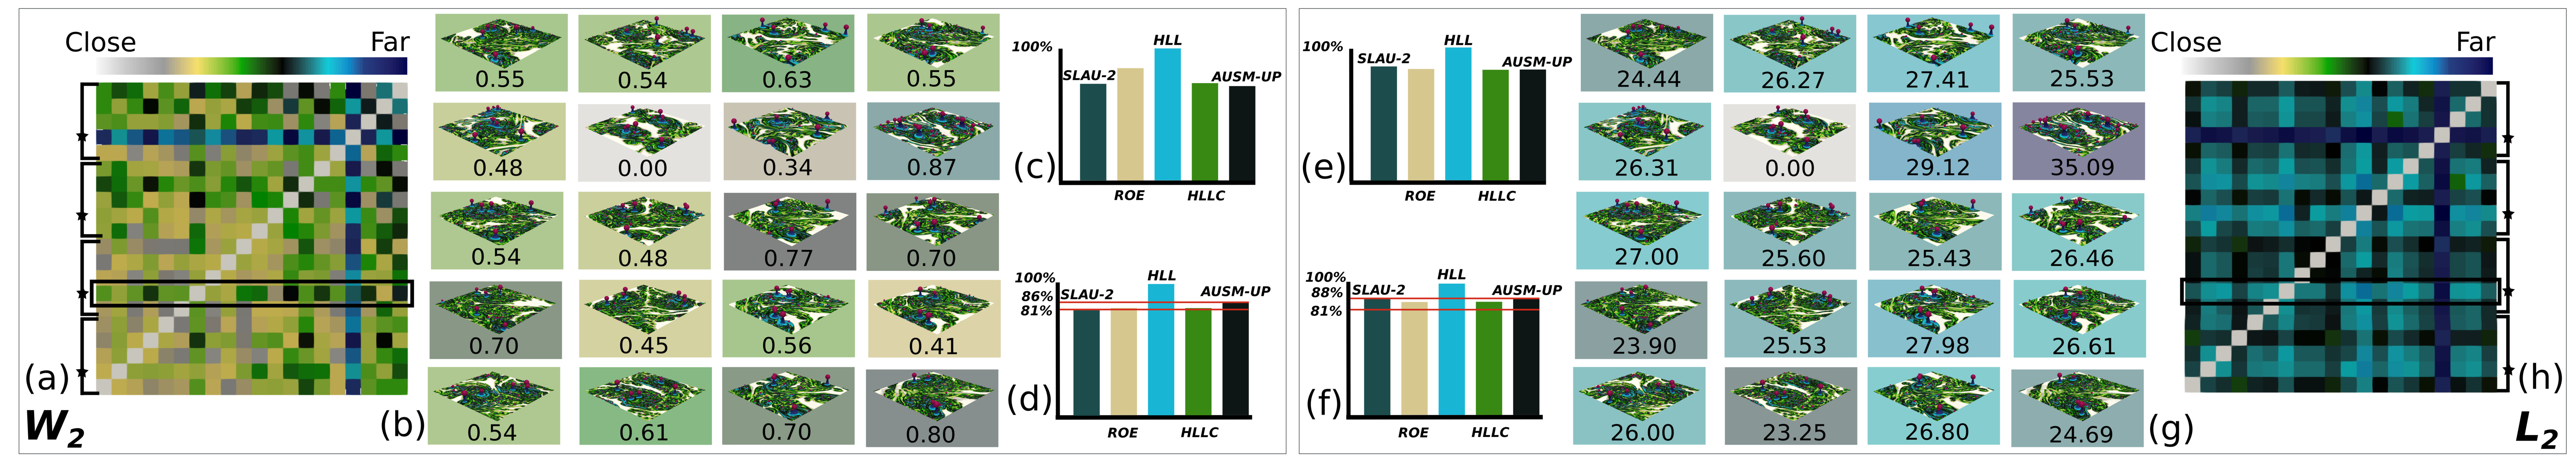
\includegraphics[width=\figureShrink\linewidth]{chapter4_topology_data_analysis/pictures/KHI_distance_to_the_rest.jpg}
 \mycaption{Comparison between the $\wasserstein{2}$ metric (left) and the standard $L_2$-metric (right) for isolating the HLL solver.
 (a,h) Distance matrix for 20 configurations at $t_2$ at $512 \times 512$. Black frames represent the distance between the TENO 7$_{th}$ order with the HLL (matrix lines marked by $\star$) and the other configurations (b,g). Histograms (c,e) are respectively the percentage average of the sum distance matrix of (a,h). Histograms (d,f) are respectively the percentage of the sum distance for all variations.}
 \label{fig_KHIdistance}
\end{figure*}


\subsection{Outlier distance profile}
\label{sec_outlier}
With this protocol (illustrated on toy examples,
\autoref{gaussian_distance}), we want to validate hypothesis H3 (\autoref{Hypotheses}), which means that for all the simulation configurations the HLL solver will be very different from other solvers to describe the Kelvin-Helmholtz instabilities. For this protocol, we take 5 simulation configurations where we fix the reconstruction (TENO or WENO-Z), the physical time ($t_0$, $t_1$, $t_2$), the mesh ($256\times 256, 512\times 512, 1024\times 1024$), the order (5 or 7) and we vary the solvers. The 5 different computations describing the same turbulent flow obtained with the solvers (HLL, SLAU2, AUSM$^+$-UP, HLLC and Roe) are analyzed regarding to the enstrophy.

A distance is used to compare the topology of the enstrophy. Many methods can be used to compute such a distance but in this protocol we focus on 2 metrics: the $L_2$-norm distance directly on the values of the enstrophy and the Wasserstein distance on the persistence diagrams. One can inject other distances if needed. For the Wasserstein, the saddle-maximum persistence diagram is computed on each result. Then, they are grouped in a unique dataset to compute a persistence diagram distance matrix (\autoref{gaussian_distance}). For the $L_2$-norm, a distance matrix  is also created where a line corresponds to the distance in the enstrophy field from one solver to the others.





Thus, the sum of the distances from one solver to the others is computed by
summing the distances on one line of the matrix. The total distance of one 
solver to the others, for all configurations, is simply the sum of all these sum 
distances for every line of the matrix which correspond to the same solver. We 
finally obtain one global distance per solver for all configurations. Finally 
the difference between the distance of the HLL and the distance of the maximizer 
(the second value if HLL is the maximum) gives a separation score. If the
difference is positive, then hypothesis H3 is verified whereas it is not if 
negative, because it means that another solver generates a flow topologically 
more different than the HLL. 
With this protocol, best separations are obtained for high absolute values.
% of 
% the score.

% the higher is the absolute value of the score, the 
% better the separation is.
% with this protocol.



\subsection{Unsupervised classification}
\label{sec_unsupervised}


With the last protocol (illustrated on toy examples in \autoref{gaussian_cluster}),
we want to validate hypotheses H4 and H5 (\autoref{Hypotheses}). We want to verify that the
simulations with the Roe and HLLC solvers are topologically close (hypothesis H4) and the
simulations with the AUSM$^+$-UP and SLAU2 solvers are topologically close (hypothesis H5). To do so, three clustering methods will be used based on Wasserstein distances and the L$_2$- norm(\autoref{sec_topology}).

For the first two clustering methods, we start by computing distance matrix with the protocol of the outlier distance profile \autoref{sec_outlier} using successively the Wasserstein distance and $L_2$-norm matrices (\autoref{gaussian_cluster}a). We apply a dimension reduction to project the distances of the matrix according to 2 components (\autoref{sec_topology}). This projection is used to generate clusters of the matrices with a k-means algorithm (\autoref{sec_topology}) as illustrated on \autoref{gaussian_cluster}b. The third clustering method uses directly the persistence diagrams(\autoref{sec_topology}) without using the distance matrix. All the persistence diagrams are merge into a single dataset to compute the Wasserstein distances between each diagram. The barycenter of persistence diagram is then used to directly compute a cluster, without dimension reduction, in the Wasserstein metric space \cite{vidal_vis19} with the ${W_2}$ distance. Then a k-means algorithm (\autoref{sec_topology}) is applied. 

With these three classification methods, we obtain different associations of our configurations. Each association is going to be scored with a measure of similarities between the clusters regarding to a reference cluster using the Rand Index \cite{rand1971objective}. This Rand index has a value between 0 and 1, with 0 indicating that two clusters do not agree on any pair of points and 1 indicating that the data clusters are exactly the same. Based on the properties of the solvers used in the simulation code HYPERION and detailed in \autoref{sec_solvers}, we define our reference cluster such that the first partition contains the AUSM$^+$-UP and SLAU2 solvers, the second partition the HLLC and Roe solvers and the third partition the HLL solver. The Rand Index is computed for each configuration and averaged per clustering method.
This
% metric
enables the
% precise
ranking of
% allows us to precisely rank
the different solver
behaviors.
% of our solvers.
If the average Rand Index score is close to 1 then both hypotheses H4, showing similarity between the AUSM$^+$-UP and SLAU2 solvers and H5, showing the isolation of the HLL solver, are verified.













\section{Results}
\label{sec_experimentalResults}
This section presents our experimental results and their interpretations, for
the protocols presented in \autoref{sec_protocols}, applied on the ensemble data
described in \autoref{sec_caseStudy}
% , which has been made
(publicly
available \cite{data}).


\subsection{Persistence curve study}



We applied protocol 1 using the persistence curves, on our ensemble dataset of Kelvin-Helmotlz instability (KHI) to verify the hypotheses of separation of the schemes (H1) and the independence of the orders (H2)(\autoref{Hypotheses}). 
The input parameters are setup as detailed in \autoref{sec_protocols}, generating 36 studies. The terrains and curves on
% Figure
\autoref{curv} illustrate the result for one configuration with a 5th order WENO-Z (\autoref{curv}.a), a 7th order WENO-Z (\autoref{curv}.c), a 5th order WENO-Z (\autoref{curv}.f) and a 5th order TENO (\autoref{curv}.h). For the scheme comparison, most of the averaged persistence curves for the TENO schemes (blue curves on \autoref{curv}g) are above the WENO-Z curves (green curves on \autoref{curv}g).
The integral difference, between the average curves, obtain results between $[-5.6,5.2]$ (\autoref{curv}.e), which demonstrates differences on the topology of the enstrophy between the interpolation methods as expected.
Hypothesis H1 is verified on the KHI ensemble dataset. For the study on the 
independence of orders, we see that the averaged persistence curves are often 
close (\autoref{curv}b). However the integral differences obtained for this 
study show larger values for the WENO-Z, \emph{i.e} in between $[-0.5, 8.1]$ 
(\autoref{curv}.d). This analysis highlights that orders play a more important 
role, in terms of topology of the vortices, for WENO-Z than for TENO. Moreover, 
we observe that this difference tends to increase at $t_2$ for both studies 
confirming that the flow is composed of a larger number of vortex as the 
simulation evolves. Hypothesis H2 is verified for the TENO solvers but not for 
the WENO-Z
% as discussed
% later 
% in
(\autoref{insights}).
 



\subsection{Outlier distance profile study}
\label{sec_KHIdistance}


% In order t
To verify the HLL isolation states in hypothesis H3 (\autoref{Hypotheses}) on our ensemble dataset, we implemented our protocol 2 (\autoref{sec_protocols}) based on the Wasserstein distance and the $L_2$-norm (\autoref{sec_topology}). For this study we apply protocol 2 where the time and the resolution are fixed. The parameters that vary are the schemes ($\times 2$), the orders ($\times 2$) and the solvers ($\times 5$) (\autoref{tab_parameters}) thus generating 20 cases. All the distances have been computed according to the protocol of the outlier distance profile. These distances are represented by a global distance matrix where a line represents the 20 configurations (Wasserstein \autoref{fig_KHIdistance}.a and $L_2-$norm \autoref{fig_KHIdistance}.h) compared to a the HLL solver choosen as the reference. The matrix view of \autoref{fig_KHIdistance}b and \autoref{fig_KHIdistance}g show the KHI terrains and the distances of all configurations to the HLL solver.

The study has been done for all time steps and all resolutions generating nine
$20\times 20$ 
distance matrices, for each distance. The histograms (Figs. 
\ref{fig_KHIdistance}.c and \ref{fig_KHIdistance}.e) 
% (\autoref{fig_KHIdistance}.c) and (\autoref{fig_KHIdistance}.e) 
show the average 
of these nine distance matrices for the Wasserstein distance and the 
$L_2$-norm, expressed in terms of percentage according to the distance of HLL 
to the other solvers (HLL being the reference at 100\%). In this case the 
percentage difference in distances to HLL are about 18\% 
(\autoref{fig_KHIdistance}.d) for the Wasserstein and 13\% for the $L_2$ 
(\autoref{fig_KHIdistance}.f). These large percentages confirm that HLL is a 
solver that behaves differently from others.
% More precisely, a
As it does not take
into account contact discontinuities, the interfaces between the vortices
are much less defined than with the other solvers, resulting in a different
number of vortices. From a physical point of view, this result confirms the 
isolation of HLL in all cases. From a topological point of view, it shows that 
the Wasserstein distance is the best at differentiating the HLL solver from the 
others (the distance gap is always bigger than the $L_2$). For this large study 
of 18 distance matrices $20\times 20$, the hypothesis H3 is verified. 

\begin{figure*}
 \centering % avoid the use of \begin{center}...\end{center} and use \centering
 \vspace{-1ex}
 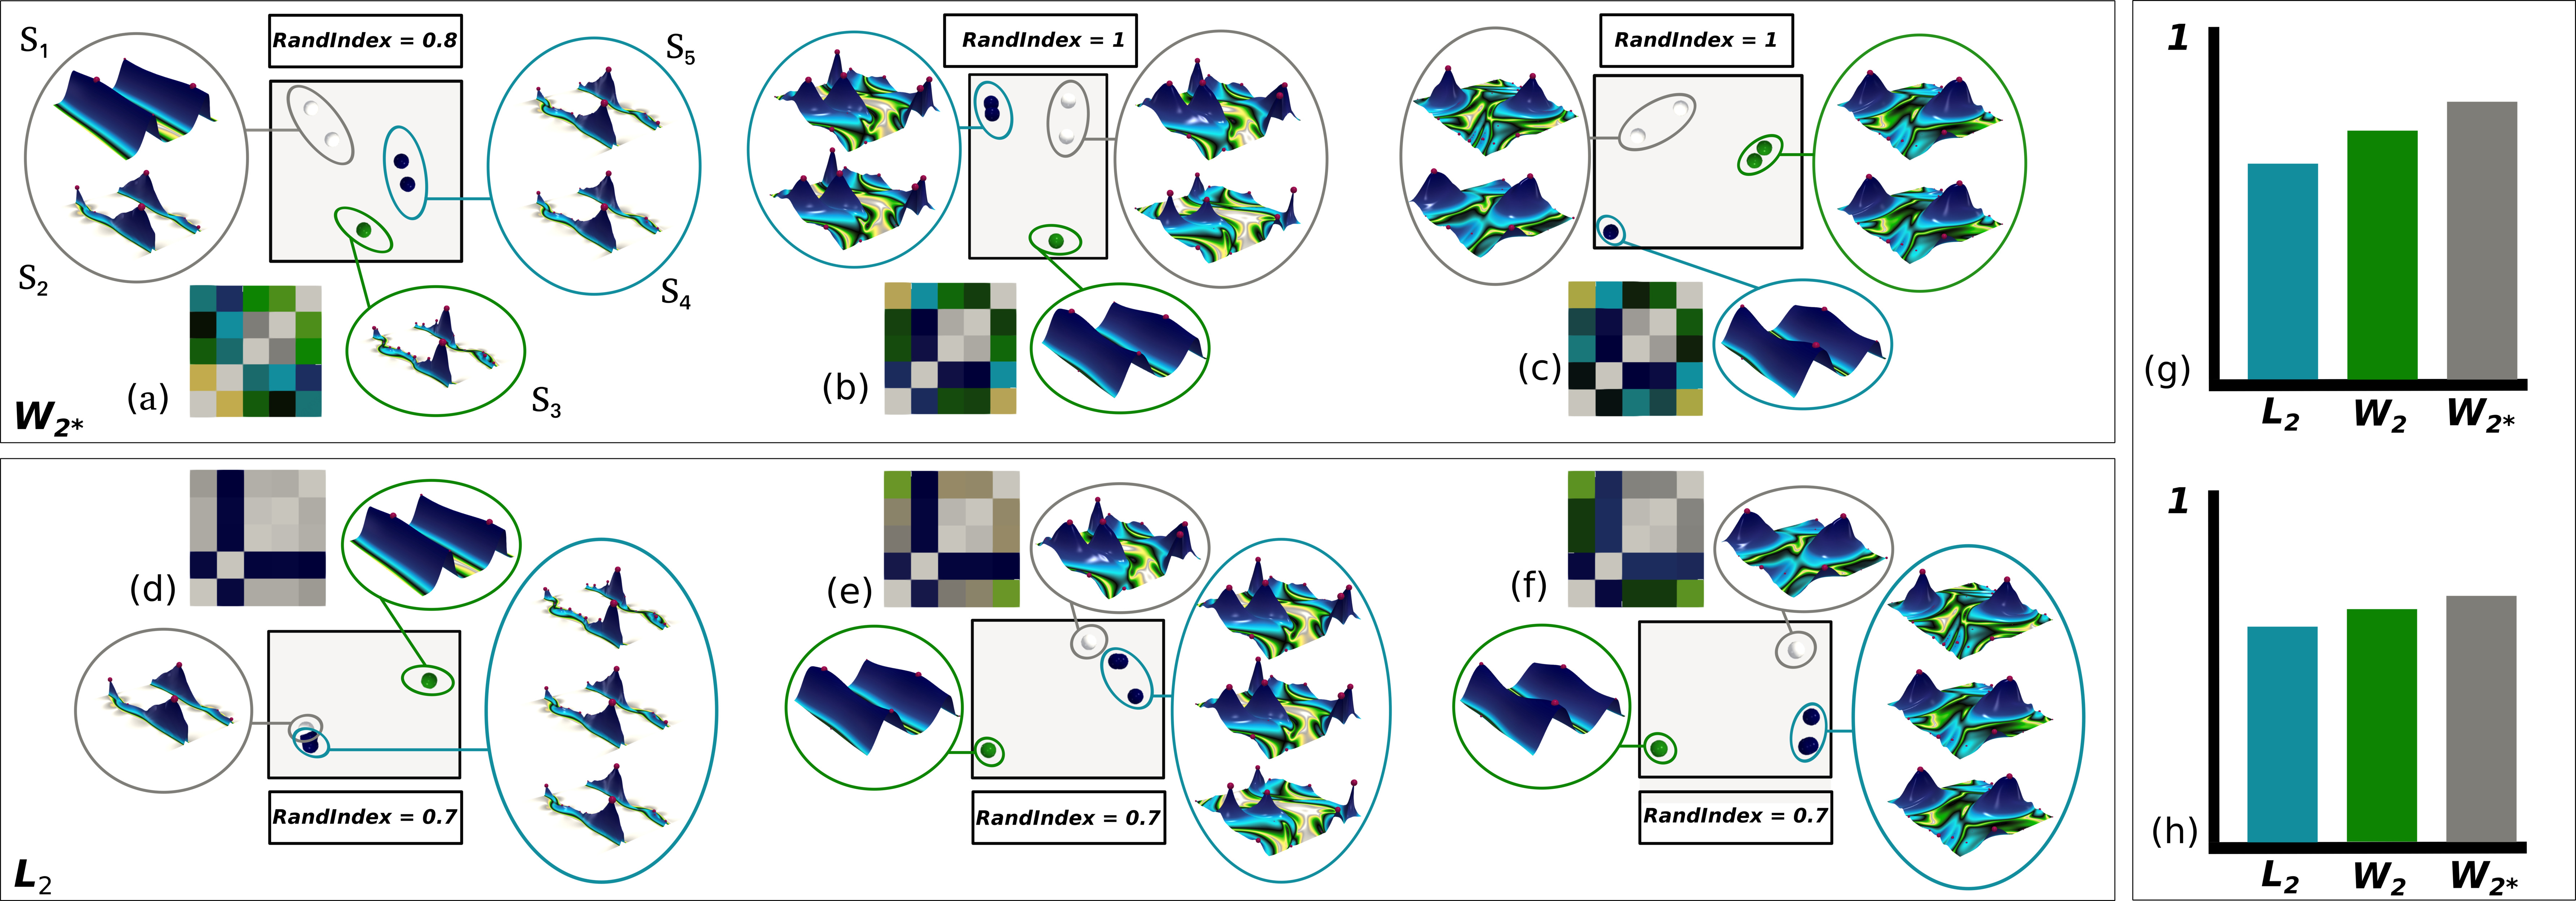
\includegraphics[width=\figureShrink\linewidth]{chapter4_topology_data_analysis/pictures/KHI_cluster.jpg}
 \mycaption{Comparison between the clustering on the Wasserstein metric space \cite{vidal_vis19} (top frame) and a clustering based on the traditional $L_2$ norm (bottom frame) for distinguishing FDS solvers from FTS solvers.
Point clouds at $t_0$, $t_1$,$t_2$ with a first order scheme at $256\times 256$.
The point cloud is a representation of the five scalar-fields in the distance
space colored according to the clusters obtained. The Rand Index are computed
with the five configurations $S_1$ (SLAU2), $S_2$ (HLL), $S_3$ (AUSM$^+$-UP),
$S_4$ (Roe), $S_5$ (HLLC). (g,h) Average Rand Index for all variations for the
high orders (bottom) and the first order (top).}
\label{fig_khi_cluster}
\end{figure*}


\subsection{Unsupervised classification study}
 \label{sec_khi_cluster}
To improve our understanding on the behavior of the solvers into our simulation code, we implemented protocol 3 on the unsupervised classification (\autoref{sec_protocols}) to verified the hypotheses H4 and H5 (\autoref{Hypotheses}). The goal is to identify the separation of FDS type solvers from the FTS type solvers (\autoref{sec_solvers}). We are interested in the low Mach reconstructions (\autoref{sec_solvers}). The challenge comes from the fact that small vortices are reconstructed on only a few cells. So, we implemented protocol 3 with the distances and clustering method detailed in \autoref{sec_protocols} leading to 5 simulation configurations (\autoref{tab_parameters}) with variable solvers. To focus on the small vortices we used a threshold of 0.38 persistence for the topological methods. On the KHI ensemble, we generated 36 clusters from the threshold persistence diagrams and obtain the Rand Index for all of them. \autoref{fig_khi_cluster}.a, \autoref{fig_khi_cluster}.b, \autoref{fig_khi_cluster}.c show the $W_2*$ clustering for the three timesteps and \autoref{fig_khi_cluster}.d, \autoref{fig_khi_cluster}.e, \autoref{fig_khi_cluster}.f for the $L_2$.

Histogram \autoref{fig_khi_cluster}.h shows the average Rand Index for the 
three methods with a value of 0.63 for $L_2$, 0.66 for $W_2$ and 0.71 for $W_2*$.
There is very little difference between the topological and geometric results 
and each of the methods struggles to get the right cluster. Hypotheses H4 and H5 
are not verified for high orders. However, to highlight the differences between 
solvers, it is necessary to use a reference reconstruction that barely captures 
small scale turbulence due to order dissipation (\autoref{sec_solvers}).
Thus, we applied protocol 3 (\autoref{sec_protocols}) on a more restricted 
dataset at order 1. Histogram \autoref{fig_khi_cluster}.g shows the average 
Rand 
Index at order 1 with the three methods leading to 0.63 for $L_2$, 0.71 for $W_2$
and 0.78 for $W_2*$. In this case, we notice that for any reconstruction, the 
topological methods obtain better clustering. Moreover, the study with order 1 
shows that the $W_2*$ method enhances solver isolation.
% of the solvers.
With this
high score of the Rand Index hypotheses H4 and H5 are verified with the first 
order. 

\subsection{Unanticipated insights}
\label{insights}

During the analysis of the persistence curves generated by our protocol 1, we found significant differences on the topology of the enstrophy between the orders for the WENO-Z. By increasing the order, we increase the accuracy of our calculation that generates more structures into the turbulent flow. On the other hand, there is no difference between the orders obtained with the TENO. This means that other ingredients in the TENO reconstruction play an important role in the computation of the turbulence such as the separation of the scales. In addition, the persistence curves also allowed us to observe that the WENO-Z schemes produce more numerical errors than the TENO. As presented in \autoref{sec_khi_cluster}, H4 and H5 hypotheses have not been verified for high orders. This means that the topological analysis does not capture the differences between the solvers. This may be due to the reconstructions which are accurate enough to calculate all velocities in the Kelvin-Helmholtz instability. 

\subsection{Limitations}
As discussed in \autoref{sec_KHIdistance}, in comparison to the $L_2$ norm, the Wasserstein distance
improvesthe separation of the HLL solver, but only by $5 \%$ (distance difference percentage). While this improvement may seem marginal, we would like to stress its significance given such challenging data,in particular with regard to the traditional approach based on kinetic energy, shown \autoref{energie}, where the five solvers can hardly be distinguished from each other.

Similarly, we can see that the Rand Index score for the three clustering
methods detailed in \autoref{sec_khi_cluster} are quite close to each other as
illustrated on \autoref{fig_khi_cluster}.h. These close scores are due to the 
interpolations schemes (\autoref{sec_simulation}) which cover up the differences 
between the different solvers.
In other words, the variations in vortex distributions induced by the choice of solver are too subtle, given the importance of the interpolation order on the outcome. As shown in \autoref{fig_khi_cluster} (top), we were still able to overcome this limitation by considering a
reconstruction that is not dedicated to turbulence, \emph{i.e.} an upwind scheme 
of order 1. This enabled us to exaggerate the impact of the solvers, thereby allowing us to
validate hypotheses H4 and H5 as reported in \autoref{sec_khi_cluster}.


\section{Conclusion}
In this paper, we have presented an experimental protocol for the comparison of
numerical methods on a Kelvin-Helmholtz instability using topological analysis.
An ensemble dataset of 180 members has been computed for this instability by a
simulation code developed in our institution and running on a supercomputer.
While traditional approaches based on the kinetic energy (\autoref{energie}) only enable
to validate the physical conformity of the generated flow,
% to assess the physical conformity of the generated flow,
our overall approach provides finer analyses. In particular,
% Based on the assumptions made in the literature (\autoref{sec_simulation}),
the
protocol using the persistence curves (\autoref{sec_persistence}) allowed us to
observe differences between the TENO and WENO-Z reconstructions. It also
confirms an independence of the
reconstruction order (5 or 7) when
using the TENO scheme allowing
% speedup
practical
computational speedup,
without loss of precision. The protocol
based on the Wasserstein distance (\autoref{sec_outlier}) succeeded in
discriminating the HLL solvers from other configurations, validating the use of
such a topological analysis to confirm domain field expectations. The last
protocol, based on recent clustering methods (\autoref{sec_khi_cluster})
successfully differentiates the topology of computations based on FDS (Flux
Difference Splitting) and FTS (Flux Type Splitting) solvers.
Overall, the validation of the hypotheses reported by CFD experts (\autoref{sec_hypotheses}) provides reliable indications for the tuning of a flow simulation, to help CFD users achieve the best balance between computation accuracy and speed.
%
%
% in contrast to traditional approaches (\autoref{energie}), which only validate the physical plausibility of a flow, our framework enabled the validation of the above hypotheses (formalized in \autoref{sec_hypotheses})}
% In particular, the validation of these hypotheses are a practical contribution towards }
% Flux Differe
% (FDS) and FTS solver computations.


The results obtained in this experimental study also show
the viability of topological methods for the representation and comparison of
Kelvin-Helmholtz
instabilities.
%
% that
%
% we can take confidence in the topological treatment for a Kelvin-Helmholtz
% instability.
The interesting aspect of these topological protocols is that the
numerical method comparisons are based on physical differences rather than on
unreliable, low-level, pointwise measures.
% quantitative.
The direction we wish to take now, for our future work, is
the extension of these protocols to 3D datasets of external hypersonics aerodynamics.
% However, in order to isolate one phenomenon on 3D data, a
% threshold study will have to be implemented. It will be necessary to decide
% which phenomenon we want to observe, such as boundary layer turbulence or
% vortices generated at the back of the hypersonic vehicle.
Another direction we
want to investigate is the evaluation of other tools used in the protocol such
as new topological distances \cite{pont_vis21} or clustering methods. Finally, this experimental
study allows us, with confidence, to consider applying these protocols to other
hydrodynamic turbulent flows studied in our institution in the domain of
hypersonic vehicle design.


% \section{Acknowledgments}
%future work:
%benchmark for other topological comparison methods.

%\section{Annexe}
\section{WENO-Z}
\subsubsection{Fifth order reconstruction, WENO5}\label{sssec:weno5}

\begin{figure}[H]
 \centering % avoid the use of \begin{center}...\end{center} and use \centering

 \includegraphics[width=\columnwidth]{stencil.png}
 \caption{Schematics illustrating the candidate stencils of seventh-order  TENO interpolation.}
 \label{fig:sample}
\end{figure}

\begin{equation}
\begin{aligned}
q_{i+1 / 2}^{l}=& w_{0}\left(\frac{1}{3} q_{i-2}-\frac{7}{6} q_{i-1}+\frac{11}{6} q_{i}\right) \\
&+w_{1}\left(-\frac{1}{6} q_{i-1}+\frac{5}{6} q_{i}+\frac{1}{3} q_{i+1}\right) \\
&+w_{2}\left(\frac{1}{3} q_{i}+\frac{5}{6} q_{i+1}-\frac{1}{6} q_{i+2}\right) \\
q_{i+1 / 2}^{R}=& w_{0}\left(\frac{1}{3} q_{i+1}+\frac{5}{6} q_{i}-\frac{1}{6} q_{i-1}\right) \\
&+w_{1}\left(-\frac{1}{6} q_{i+2}+\frac{5}{6} q_{i+1}+\frac{1}{3} q_{i}\right) \\
&+w_{2}\left(\frac{1}{3} q_{i+3}-\frac{7}{6} q_{i+2}+\frac{11}{6} q_{i+1}\right)
\end{aligned}
\end{equation}\\

$$d_0=\frac{1}{10} \quad d_1=\frac{3}{5} \quad d_2=\frac{3}{10}$$
\begin{equation}
\begin{array}{l}
w_{k}=\frac{\alpha_{k}}{\alpha_{0}+\alpha_{1}+\alpha_{2}}, \quad \alpha_{k}=d_k\left(1+\left(\frac{\tau_5}{\beta_{k}+\epsilon}\right)^2\right), \quad k=0,1,2\\
\end{array}
\end{equation}

\begin{equation}
\tau_5=\left|\beta_0-\beta_2\right|
\end{equation}

\begin{equation}
\begin{array}{l}
\beta_{0}=\frac{13}{12}\left(q_{i-2}-2 q_{i-1}+q_{i}\right)^{2}+\frac{1}{4}\left(q_{i-2}-4 q_{i-1}+3 q_{i}\right)^{2}\\
\beta_{1}=\frac{13}{12}\left(q_{i-1}-2 q_{i}+q_{i+1}\right)^{2}+\frac{1}{4}\left(q_{i-1}-q_{i+1}\right)^{2}\\
\beta_{2}=\frac{13}{12}\left(q_{i}-2 q_{i+1}+q_{i+2}\right)^{2}+\frac{1}{4}\left(3 q_{i}-4 q_{i+1}+q_{i+2}\right)^{2}
\end{array}
\end{equation}

$$d_0=\frac{3}{10} \quad d_1=\frac{3}{5} \quad d_2=\frac{1}{10}$$
\begin{equation}
\begin{array}{l}
w_{k}=\frac{\alpha_{k}}{\alpha_{0}+\alpha_{1}+\alpha_{2}}, \quad \alpha_{k}=d_k\left(1+\left(\frac{\tau_5}{\beta_{k}+\epsilon}\right)^2\right), \quad k=0,1,2\\
\end{array}
\end{equation}

\begin{equation}
\tau_5=\left|\beta_0-\beta_2\right|
\end{equation}

\begin{equation}
\begin{array}{l}
\beta_{0}=\frac{13}{12}\left(q_{i-1}-2 q_{i}+q_{i+1}\right)^{2}+\frac{1}{4}\left(q_{i-1}-4 q_{i}+3 q_{i+1}\right)^{2}\\
\beta_{1}=\frac{13}{12}\left(q_{i}-2 q_{i+1}+q_{i+2}\right)^{2}+\frac{1}{4}\left(q_{i}-q_{i+2}\right)^{2}\\
\beta_{2}=\frac{13}{12}\left(q_{i+1}-2 q_{i+2}+q_{i+3}\right)^{2}+\frac{1}{4}\left(3 q_{i+1}-4 q_{i+2}+q_{i+3}\right)^{2}
\end{array}
\end{equation}

\subsection{WENO-Z 7}
\begin{equation}
\begin{aligned}
q_{i+1 / 2}^{l}=& w_{0}\left(-\frac{1}{4} q_{i-3}+\frac{13}{12} q_{i-2}-\frac{23}{12} q_{i-1}+\frac{25}{12} q_{i}\right) \\
&+w_{1}\left(\frac{1}{12} q_{i-2}-\frac{5}{12} q_{i-1}+\frac{13}{12} q_{i}+\frac{1}{4} q_{i+1}\right) \\
&+w_{2}\left(-\frac{1}{12} q_{i-1}+\frac{7}{12} q_{i}+\frac{7}{12} q_{i+1}-\frac{1}{12} q_{i+2}\right) \\
&+w_{3}\left(\frac{1}{4} q_{i}+\frac{13}{12} q_{i+1}-\frac{5}{12} q_{i+2}+\frac{1}{12} q_{i+3}\right)
\end{aligned}
\end{equation}

\begin{equation}
\begin{aligned}
q_{i+1 / 2}^{R}=& w_{0}\left(\frac{1}{4} q_{i+1}+\frac{13}{12} q_{i}-\frac{5}{12} q_{i-1}+\frac{1}{12} q_{i-2}\right) \\
&+w_{1}\left(-\frac{1}{12} q_{i+2}+\frac{7}{12} q_{+1}+\frac{7}{12} q_{i}-\frac{1}{12} q_{i-1}\right) \\
&+w_{2}\left(\frac{1}{12} q_{i+3}-\frac{5}{12} q_{i+2}+\frac{13}{12} q_{i+1}+\frac{1}{4} q_{i}\right) \\
&+w_{3}\left(-\frac{1}{4} q_{i+4}+\frac{13}{12} q_{i+3}-\frac{23}{12} q_{i+2}+\frac{25}{12} q_{i+1}\right)
\end{aligned}
\end{equation}

$$d_0=\frac{1}{35} \quad d_1=\frac{12}{35} \quad d_2=\frac{18}{35} \quad d_3=\frac{4}{35}$$
\begin{equation}
\begin{array}{l}
w_{k}=\frac{\alpha_{k}}{\alpha_{0}+\alpha_{1}+\alpha_{2}}, \quad \alpha_{k}=d_k\left(1+\left(\frac{\tau_7}{\beta_{k}+\epsilon}\right)^2\right), \quad k=0,1,2\\
\end{array}
\end{equation}

\begin{equation}
\tau_7=\left|\beta_0+3\beta_1-3\beta_2-\beta3\right|
\end{equation}

\begin{equation}
\begin{aligned}
\beta_{0}=& q_{i-3}\left(547 q_{i-3}-3882 q_{i-2}+4642 q_{i-1}-1854 q_{i}\right) \\
&+q_{i-2}\left(7043 q_{i-2}-17246 q_{i-1}+7042 q_{i}\right) \\
&+q_{i-1}\left(11003 q_{i-1}-9402 q_{i}\right)+q_{i}\left(2107 q_{i}\right)
\end{aligned}
\end{equation}

\begin{equation}
\begin{aligned}
\beta_{1}=& q_{i-2}\left(267 q_{i-2}-1642 q_{i-1}+1602 q_{i}-494 q_{i+1}\right) \\
&+q_{i-1}\left(2843 q_{i-1}-5966 q_{i}+1922 q_{i+1}\right)\\
&+q_{i}\left(3443 q_{i}-2522 q_{i+1}\right)+q_{i+1}\left(547 q_{i+1}\right)
\end{aligned}
\end{equation}

\begin{equation}
\begin{aligned}
\beta_{2}=& q_{i-1}\left(547 q_{i-1}-2522 q_{i}+1922 q_{i+1}-494 q_{i+2}\right) \\
&+q_{i}\left(3443 q_{i}-5966 q_{i+1}+1602 q_{i+2}\right) \\
&+q_{i+1}\left(2843 q_{i+1}-1642 q_{i+2}\right)+q_{i+2}\left(267 q_{i+2}\right)
\end{aligned}
\end{equation}

\begin{equation}
\begin{aligned}
\beta_{3}=& q_{i}\left(2107 q_{i}-9402 q_{i+1}+7042 q_{i+2}-1854 q_{i+3}\right) \\
&+q_{i+1}\left(11003 q_{i+1}-17246 q_{i+2}+4642 q_{i+3}\right) \\
&+q_{i+2}\left(7043 q_{i+2}-3882 q_{i+3}\right)+q_{i+3}\left(547 q_{i+3}\right)
\end{aligned}
\end{equation}

$$d_0=\frac{4}{35} \quad d_1=\frac{18}{35} \quad d_2=\frac{12}{35} \quad d_3=\frac{1}{35}$$
\begin{equation}
\begin{array}{l}
w_{k}=\frac{\alpha_{k}}{\alpha_{0}+\alpha_{1}+\alpha_{2}}, \quad \alpha_{k}=d_k\left(1+\left(\frac{\tau_7}{\beta_{k}+\epsilon}\right)^2\right), \quad k=0,1,2\\
\end{array}
\end{equation}

\begin{equation}
\tau_7=\left|\beta_0+3\beta_1-3\beta_2-\beta3\right|
\end{equation}

\begin{equation}
\begin{aligned}
\beta_{0}=& q_{i-2}\left(547 q_{i-2}-3882 q_{i-1}+4642 q_{i}-1854 q_{i+1}\right) \\
&+q_{i-1}\left(7043 q_{i-1}-17246 q_{i}+7042 q_{+1}\right) \\
&+q_{i}\left(11003 q_{i}-9402 q_{i+1}\right)+q_{i+1}\left(2107 q_{i+1}\right)
\end{aligned}
\end{equation}

\begin{equation}
\begin{aligned}
\beta_{1}=& q_{i-1}\left(267 q_{i-1}-1642 q_{i}+1602 q_{i+1}-494 q_{i+2}\right) \\
&+q_{i}\left(2843 q_{i}-5966 q_{i+1}+1922 q_{i+2}\right)\\
&+q_{i+1}\left(3443 q_{i+1}-2522 q_{i+2}\right)+q_{i+2}\left(547 q_{i+2}\right)
\end{aligned}
\end{equation}

\begin{equation}
\begin{aligned}
\beta_{2}=& q_{i}\left(547 q_{i}-2522 q_{i+1}+1922 q_{i+2}-494 q_{i+3}\right) \\
&+q_{i+1}\left(3443 q_{i+1}-5966 q_{i+2}+1602 q_{i+3}\right) \\
&+q_{i+2}\left(2843 q_{i+2}-1642 q_{i+3}\right)+q_{i+3}\left(267 q_{i+3}\right)
\end{aligned}
\end{equation}

\begin{equation}
\begin{aligned}
\beta_{3}=& q_{i+1}\left(2107 q_{i+1}-9402 q_{i+2}+7042 q_{i+3}-1854 q_{i+4}\right) \\
&+q_{i+2}\left(11003 q_{i+2}-17246 q_{i+3}+4642 q_{i+4}\right) \\
&+q_{i+3}\left(7043 q_{i+3}-3882 q_{i+4}\right)+q_{i+34}\left(547 q_{i+4}\right)
\end{aligned}
\end{equation}


\subsection{TENO reconstruction schemes}

\subsubsection{Fifth order reconstruction, TENO5}

\begin{equation}
\begin{aligned}
q_{i+1 / 2}^{l}=& w_{0}\left(-\frac{1}{6} q_{i-1}+\frac{5}{6} q_{i}+\frac{2}{6} q_{i+1}\right) \\
&+w_{1}\left(\frac{2}{6} q_{i}+\frac{5}{6} q_{i+1}-\frac{1}{6} q_{i+2}\right) \\
&+w_{2}\left(\frac{2}{6} q_{i-2}-\frac{7}{6} q_{i-1}+\frac{11}{6} q_{i}\right) \\
\end{aligned}
\end{equation}

\begin{equation}
\begin{array}{l}
\beta_{0}=\frac{13}{12}\left(q_{i-1}-2 q_{i}+q_{i+1}\right)^{2}+\frac{1}{4}\left(q_{i-1}-q_{i+1}\right)^{2}\\
\beta_{1}=\frac{13}{12}\left(q_{i}-2 q_{i+1}+q_{i+2}\right)^{2}+\frac{1}{4}\left(3 q_{i}-4 q_{i+1}+q_{i+2}\right)^{2}\\
\beta_{2}=\frac{13}{12}\left(q_{i-2}-2 q_{i-1}+q_{i}\right)^{2}+\frac{1}{4}\left(q_{i-2}-4 q_{i-1}+3 q_{i}\right)^{2}\\
\end{array}
\end{equation}

\begin{equation}
\gamma_{k}=\left(1+\frac{\tau_{5}}{\beta_{k}+\varepsilon}\right)^{2}, k=0, \ldots, 2
\end{equation}

\begin{equation}
\tau_{5}=\left|\beta_{5}-\frac{1}{6}\left(\beta_{1}+\beta_{2}+4 \beta_{0}\right)\right|=O\left(\Delta x^{6}\right)
\end{equation}

\begin{equation}
\begin{aligned}
\beta_{5}&=\frac{1727}{1260}q_{i-2}^2+(67923q_i -51001q_{i-1} -38947q_{i+1}+8209q_{i+2})\frac{q_{i-2}}{5040}\\
&+\frac{104963}{5040}q_{i-1}^2+(-299076q_{i}+179098q_{i+1}-38947q_{i+2})\frac{q_{i-1}}{5040}\\
&+\frac{104963}{5040}q_{i+1}^2+(-299076q_{i}-51001q_{i+2})\frac{q_{i+1}}{5040}\\
&+\frac{77051}{1680}q_{i}^2+\frac{7547}{560}q_{i+2}q_{i}+\frac{1727}{1260}q_{i+2}^2
\end{aligned}
\end{equation}
% cg2 = 0.1727e4 / 0.1260e4 * pow(f_(i - 2), 2) + (67923 * f_i - 51001 * f_(i - 1) - 38947 * f_(i + 1) + 8209 * f_(i + 2)) * f_(i - 2) / 5040 + 0.104963e6 / 0.5040e4 * (int) pow((double) f_(i - 1), (double) 2) + (-299076 * f_i + 179098 * f_(i + 1) - 38947 * f_(i + 2)) * f_(i - 1) / 5040 + 0.104963e6 / 0.5040e4 * (int) pow((double) f_(i + 1), (double) 2) + (-299076 * f_i - 51001 * f_(i + 2)) * f_(i + 1) / 5040 + 0.77051e5 / 0.1680e4 * f_i * f_i + 0.7547e4 / 0.560e3 * f_(i + 2) * f_i + 0.1727e4 / 0.1260e4 * (int) pow((double) f_(i + 2), (double) 2);
\begin{equation}
\chi_{k}=\frac{\gamma_{k}}{\sum_{k=0}^{2} \gamma_{k}}
\end{equation}

\begin{equation}
\delta_{k}=\left\{\begin{array}{ll}
0, & \text { if } \chi_{k}<C_{T} \\
1, & \text { otherwise }
\end{array}\right.
\end{equation}

$$d_0=\frac{6}{10} \quad d_1=\frac{3}{10} \quad d_2=\frac{1}{10}$$
\begin{equation}
\begin{array}{l}
w_{k}=\frac{\alpha_{k}}{\sum_{k=0}^{2} \alpha_{k}}, \quad \alpha_{k}=d_k\delta_k, \quad k=0,1,2\\
\end{array}
\end{equation}

\begin{equation}
\begin{aligned}
q_{i+1 / 2}^{r}=& w_{0}\left(\frac{2}{6} q_{i}+\frac{5}{6} q_{i+1}-\frac{1}{6} q_{i+2}\right) \\
&+w_{1}\left(-\frac{1}{6} q_{i-1}+\frac{5}{6} q_{i}+\frac{2}{6} q_{i+1}\right) \\
&+w_{2}\left(\frac{11}{6} q_{i+1}-\frac{7}{6} q_{i+2}+\frac{2}{6} q_{i+3}\right) \\
\end{aligned}
\end{equation}

\begin{equation}
\begin{array}{l}
\beta_{0}=\frac{13}{12}\left(q_{i}-2 q_{i+1}+q_{i+2}\right)^{2}+\frac{1}{4}\left(q_{i}-q_{i+2}\right)^{2}\\
\beta_{1}=\frac{13}{12}\left(q_{i-1}-2 q_{i}+q_{i+1}\right)^{2}+\frac{1}{4}\left(q_{i-1}-4 q_{i}+q_{i+1}\right)^{2}\\
\beta_{2}=\frac{13}{12}\left(q_{i+1}-2 q_{i+2}+q_{i+3}\right)^{2}+\frac{1}{4}\left(3q_{i+1}-4 q_{i+2}+q_{i+3}\right)^{2}\\
\end{array}
\end{equation}

\begin{equation}
\gamma_{k}=\left(1+\frac{\tau_{5}}{\beta_{k}+\varepsilon}\right)^{2}, k=0, \ldots, 2
\end{equation}

\begin{equation}
\tau_{5}=\left|\beta_{5}-\frac{1}{6}\left(\beta_{1}+\beta_{2}+4 \beta_{0}\right)\right|=O\left(\Delta x^{6}\right)
\end{equation}

\begin{equation}
\begin{aligned}
\beta_{5}&=\frac{1727}{1260}q_{i-1}^2+(-51001q_{i}+67923q_{i+1} -38947q_{i+2}+8209q_{i+3})\frac{q_{i-1}}{5040}\\
&+\frac{77051}{1680}q_{i+1}^2+(-299076q_{i}-299076q_{i+2}+67923q_{i+3})\frac{q_{i+1}}{5040}\\
&+\frac{104963}{5040}q_{i+2}^2+(179098q_{i}-51001q_{i+3})\frac{q_{i+2}}{5040}\\
&+\frac{104963}{5040}q_{i}^2-\frac{38947}{5040}q_{i+3}q_{i}+\frac{1727}{1260}q_{i+3}^2
\end{aligned}
\end{equation}
% cg6 = 0.1727e4 / 0.1260e4 * pow(f_(i - 1), 2) + (-51001 * f_i + 67923 * f_(i + 1) - 38947 * f_(i + 2) + 8209 * f_(i + 3)) * f_(i - 1) / 5040 + 0.77051e5 / 0.1680e4 * (int) pow((double) f_(i + 1), (double) 2) + (-299076 * f_i - 299076 * f_(i + 2) + 67923 * f_(i + 3)) * f_(i + 1) / 5040 + 0.104963e6 / 0.5040e4 * (int) pow((double) f_(i + 2), (double) 2) + (179098 * f_i - 51001 * f_(i + 3)) * f_(i + 2) / 5040 + 0.104963e6 / 0.5040e4 * f_i * f_i - 0.38947e5 / 0.5040e4 * f_(i + 3) * f_i + 0.1727e4 / 0.1260e4 * (int) pow((double) f_(i + 3), (double) 2);
\begin{equation}
\chi_{k}=\frac{\gamma_{k}}{\sum_{k=0}^{2} \gamma_{k}}
\end{equation}

\begin{equation}
\delta_{k}=\left\{\begin{array}{ll}
0, & \text { if } \chi_{k}<C_{T} \\
1, & \text { otherwise }
\end{array}\right.
\end{equation}

$$d_0=\frac{6}{10} \quad d_1=\frac{3}{10} \quad d_2=\frac{1}{10}$$
\begin{equation}
\begin{array}{l}
w_{k}=\frac{\alpha_{k}}{\sum_{k=0}^{2} \alpha_{k}}, \quad \alpha_{k}=d_k\delta_k, \quad k=0,1,2\\
\end{array}
\end{equation}

\subsubsection{Seventh order reconstruction, TENO7}

\begin{equation}
\begin{aligned}
q_{i+1 / 2}^{l}=& w_{0}\left(-\frac{1}{6} q_{i-1}+\frac{5}{6} q_{i}-\frac{2}{6} q_{i+1}\right) \\
&+w_{1}\left(\frac{2}{6} q_{i}+\frac{5}{6} q_{i+1}-\frac{1}{6} q_{i+2}\right) \\
&+w_{2}\left(\frac{2}{6} q_{i-2}-\frac{7}{6} q_{i-1}+\frac{11}{6} q_{i}\right) \\
&+w_{3}\left(\frac{3}{12} q_{i}+\frac{13}{12} q_{i+1}-\frac{5}{12} q_{i+2}+\frac{1}{12}q_{i+3}\right) \\
&+w_{4}\left(-\frac{3}{12} q_{i-3}+\frac{13}{12} q_{i-2}-\frac{23}{12} q_{i-1}+\frac{25}{12}q_{i}\right) \\
\end{aligned}
\end{equation}

\begin{equation}
\begin{aligned}
\beta_{0}&=\frac{13}{12}\left(q_{i-1}-2 q_{i}+q_{i+1}\right)^{2}+\frac{1}{4}\left(q_{i-1}-q_{i+1}\right)^{2}\\
\beta_{1}&=\frac{13}{12}\left(q_{i}-2 q_{i+1}+q_{i+2}\right)^{2}+\frac{1}{4}\left(3 q_{i}-4 q_{i+1}+q_{i+2}\right)^{2}\\
\beta_{2}&=\frac{13}{12}\left(q_{i-2}-2 q_{i-1}+q_{i}\right)^{2}+\frac{1}{4}\left(q_{i-2}-4 q_{i-1}+3 q_{i}\right)^{2}\\
\beta_{3} &=\frac{1}{240}\left[q_{i}\left(2107 q_{i}-9402 q_{i+1}+7042 q_{i+2}-1854 q_{i+3}\right)\right.\\
&+q_{i+1}\left(11003 q_{i+1}-17246 q_{i+2}+4642 q_{i+3}\right) \\
&\left.+q_{i+2}\left(7043 q_{i+2}-3882 q_{i+3}\right)+547 q_{i+3} q_{i+3}\right] \\
\beta_{4} &=\frac{1}{240}\left[q_{i-3}\left(547 q_{i-3}-3882 q_{i-2}+4642 q_{i-1}-1854 q_{i}\right)\right.\\
&+q_{i-2}\left(7043 q_{i-2}-17246 q_{i-1}+7042 q_{i}\right) \\
&\left.+q_{i-1}\left(11003 q_{i-1}-9402 q_{i}\right)+2107 q_{i} q_{i}\right]
\end{aligned}
\end{equation}

\begin{equation}
\gamma_{k}=\left(1+\frac{\tau_{7}}{\beta_{k}+\varepsilon}\right)^{2}, k=0, \ldots, 4
\end{equation}

\begin{equation}
\tau_{7}=\left|\beta_{7}-\frac{1}{6}\left(\beta_{1}+\beta_{2}+4 \beta_{0}\right)\right|=O\left(\Delta x^{6}\right)
\end{equation}

\begin{equation}
\begin{aligned}
\beta_7&=\frac{2627203}{1871100}q_{i - 2}^2 + (2283428883q_{i} - 969999969 q_{i - 1} - 2806252532 q_{i + 1} + 1902531828 q_{i + 2} - 676871859 q_{i + 3} + 99022657 q_{i + 4}) \frac{q_{i - 2}}{59875200}\\
&+ \frac{108444169}{2217600}q_{i - 1}^2 + (-14296379553  q_{i} + 18083339772 q_{i + 1} - 12546315963 q_{i + 2} + 4550242446 q_{i + 3} - 676871859  q_{i + 4}) \frac{q_{i - 1}}{59875200}\\
&+ \frac{1607739169}{2993760} q_{i + 1}^2 + (-47431870620  q_{i} - 47431870620 q_{i + 2} + 18083339772 q_{i + 3} - 2806252532  q_{i + 4})\frac{q_{i + 1}}{59875200} \\
&+ \frac{16790707}{55440} q_{i + 2}^2 (33820678305 q_{i} - 14296379553 q_{i + 3} + 2283428883 q_{i + 4}) \frac{q_{i + 2}}{59875200}\\
&+ \frac{108444169}{2217600} q_{i + 3}^2 + (-12546315963 q_{i} - 969999969 q_{i + 4})\frac{q_{i + 3}}{59875200}\\
&+ \frac{16790707}{55440}q_{i}^2 + \frac{158544319}{4989600} q_{i + 4} q_{i} +\frac{2627203}{1871100} q_{i + 4}^2;
\end{aligned}
\end{equation}
%cg7 = 0.2627203e7 / 0.1871100e7 * pow(f_(i - 2), 2) + (2283428883 * f_i - 969999969 * f_(i - 1) - 2806252532 * f_(i + 1) + 1902531828 * f_(i + 2) - 676871859 * f_(i + 3) + 99022657 * f_(i + 4)) * f_(i - 2) / 59875200 + 0.108444169e9 / 0.2217600e7 * (int) pow((double) f_(i - 1), (double) 2) + (-14296379553 * f_i + 18083339772 * f_(i + 1) - 12546315963 * f_(i + 2) + 4550242446 * f_(i + 3) - 676871859 * f_(i + 4)) * f_(i - 1) / 59875200 + 0.1607739169e10 / 0.2993760e7 * (int) pow((double) f_(i + 1), (double) 2) + (-47431870620 * f_i - 47431870620 * f_(i + 2) + 18083339772 * f_(i + 3) - 2806252532 * f_(i + 4)) * f_(i + 1) / 59875200 + 0.16790707e8 / 0.55440e5 * (int) pow((double) f_(i + 2), (double) 2) + (33820678305 * f_i - 14296379553 * f_(i + 3) + 2283428883 * f_(i + 4)) * f_(i + 2) / 59875200 + 0.108444169e9 / 0.2217600e7 * (int) pow((double) f_(i + 3), (double) 2) + (-12546315963 * f_i - 969999969 * f_(i + 4)) * f_(i + 3) / 59875200 + 0.16790707e8 / 0.55440e5 * f_i * f_i + 0.158544319e9 / 0.4989600e7 * f_(i + 4) * f_i + 0.2627203e7 / 0.1871100e7 * (int) pow((double) f_(i + 4), (double) 2);
\begin{equation}
\chi_{k}=\frac{\gamma_{k}}{\sum_{k=0}^{4} \gamma_{k}}
\end{equation}

\begin{equation}
\delta_{k}=\left\{\begin{array}{ll}
0, & \text { if } \chi_{k}<C_{T} \\
1, & \text { otherwise }
\end{array}\right.
\end{equation}

$$d_0=\frac{18}{35} \quad d_1=\frac{9}{35} \quad d_2=\frac{3}{35} \quad d_3=\frac{4}{35} \quad d_4=\frac{1}{35}$$
\begin{equation}
\begin{array}{l}
w_{k}=\frac{\alpha_{k}}{\sum_{k=0}^{4} \alpha_{k}}, \quad \alpha_{k}=d_k\delta_k, \quad k=0,1,2,3,4\\
\end{array}
\end{equation}


\begin{equation}
\begin{aligned}
q_{i+1 / 2}^{r}=& w_{0}\left(\frac{2}{6} q_{i}+\frac{5}{6} q_{i+1}-\frac{1}{6} q_{i+2}\right) \\
&+w_{1}\left(-\frac{1}{6} q_{i-1}+\frac{5}{6} q_{i}+\frac{2}{6} q_{i+1}\right) \\
&+w_{2}\left(\frac{11}{6} q_{i+1}-\frac{7}{6} q_{i+2}+\frac{2}{6} q_{i+3}\right) \\
&+w_{3}\left(\frac{1}{12} q_{i-2}-\frac{5}{12} q_{i-1}+\frac{13}{12} q_{i}+\frac{3}{12}q_{i+1}\right) \\
&+w_{4}\left(\frac{25}{12} q_{i+1}-\frac{23}{12} q_{i+2}+\frac{13}{12} q_{i+3}-\frac{3}{12}q_{i+4}\right) \\
\end{aligned}
\end{equation}

\begin{equation}
\begin{aligned}
\beta_{0}&=\frac{13}{12}\left(q_{i}-2 q_{i+1}+q_{i+2}\right)^{2}+\frac{1}{4}\left(q_{i}-q_{i+2}\right)^{2}\\
\beta_{1}&=\frac{13}{12}\left(q_{i-1}-2 q_{i}+q_{i+1}\right)^{2}+\frac{1}{4}\left(q_{i-1}-4 q_{i}+q_{i+1}\right)^{2}\\
\beta_{2}&=\frac{13}{12}\left(q_{i+1}-2 q_{i+2}+q_{i+3}\right)^{2}+\frac{1}{4}\left(3q_{i+1}-4 q_{i+2}+q_{i+3}\right)^{2}\\
\beta_{3} &=\frac{1}{240}\left[q_{i+1}\left(2107 q_{i+1}-9402 q_{i}+7042 q_{i-1}-1854 q_{i-2}\right)\right.\\
&+q_{i}\left(11003 q_{i}-17246 q_{i-1}+4642 q_{i-2}\right) \\
&\left.+q_{i-1}\left(7043 q_{i-1}-3882 q_{i-2}\right)+547 q_{i-2} q_{i-2}\right] \\
\beta_{4} &=\frac{1}{240}\left[q_{i+4}\left(547 q_{i+4}-3882 q_{i+3}+4642 q_{i+2}-1854 q_{i+1}\right)\right.\\
&+q_{i+3}\left(7043 q_{i+3}-17246 q_{i+2}+7042 q_{i+1}\right) \\
&\left.+q_{i+2}\left(11003 q_{i+2}-9402 q_{i+1}\right)+2107 q_{i+1} q_{i+1}\right]
\end{aligned}
\end{equation}

\begin{equation}
\gamma_{k}=\left(1+\frac{\tau_{7}}{\beta_{k}+\varepsilon}\right)^{2}, k=0, \ldots, 4
\end{equation}

\begin{equation}
\tau_{7}=\left|\beta_{7}-\frac{1}{6}\left(\beta_{1}+\beta_{2}+4 \beta_{0}\right)\right|=O\left(\Delta x^{6}\right)
\end{equation}

\begin{equation}
\begin{aligned}
\beta_7&=\frac{2627203}{1871100}q_{i - 3}^2 + (2283428883q_{i-1} - 969999969 q_{i - 2} - 2806252532 q_{i} + 1902531828 q_{i + 1} - 676871859 q_{i + 2} + 99022657 q_{i + 3}) \frac{q_{i - 3}}{59875200}\\
&+ \frac{108444169}{2217600}q_{i - 2}^2 + (-14296379553  q_{i-1} + 18083339772 q_{i} - 12546315963 q_{i + 1} + 4550242446 q_{i + 2} - 676871859  q_{i + 3}) \frac{q_{i - 2}}{59875200}\\
&+ \frac{1607739169}{55440} q_{i- 1}^2 + (-47431870620  q_{i} + 33820678305 q_{i + 1} -12546315963 q_{i + 2} + 1902531828  q_{i + 3})\frac{q_{i - 1}}{59875200} \\
&+ \frac{16790707}{55440} q_{i + 1}^2 (-47431870620 q_{i} - 14296379553 q_{i + 2} + 2283428883 q_{i + 3}) \frac{q_{i + 1}}{59875200}\\
&+ \frac{108444169}{2217600} q_{i + 2}^2 + (18083339772 q_{i} - 969999969 q_{i + 3})\frac{q_{i + 3}}{59875200}\\
&+ \frac{16790707}{2993760}q_{i}^2 - \frac{701563133}{14968800} q_{i + 3} q_{i} +\frac{2627203}{1871100} q_{i + 3}^2;
\end{aligned}
\end{equation}
%cg5 = 0.2627203e7 / 0.1871100e7 * pow(f_(i - 3), 2) + (-2806252532 * f_i - 969999969 * f_(i - 2) + 2283428883 * f_(i - 1) + 1902531828 * f_(i + 1) - 676871859 * f_(i + 2) + 99022657 * f_(i + 3)) * f_(i - 3) / 59875200 + 0.108444169e9 / 0.2217600e7 * (int) pow((double) f_(i - 2), (double) 2) + (18083339772 * f_i - 14296379553 * f_(i - 1) - 12546315963 * f_(i + 1) + 4550242446 * f_(i + 2) - 676871859 * f_(i + 3)) * f_(i - 2) / 59875200 + 0.16790707e8 / 0.55440e5 * (int) pow((double) f_(i - 1), (double) 2) + (-47431870620 * f_i + 33820678305 * f_(i + 1) - 12546315963 * f_(i + 2) + 1902531828 * f_(i + 3)) * f_(i - 1) / 59875200 + 0.16790707e8 / 0.55440e5 * (int) pow((double) f_(i + 1), (double) 2) + (-47431870620 * f_i - 14296379553 * f_(i + 2) + 2283428883 * f_(i + 3)) * f_(i + 1) / 59875200+ 0.108444169e9 / 0.2217600e7 * (int) pow((double) f_(i + 2), (double) 2) + (18083339772 * f_i - 969999969 * f_(i + 3)) * f_(i + 2) / 59875200 + 0.1607739169e10 / 0.2993760e7 * f_i * f_i - 0.701563133e9 / 0.14968800e8 * f_(i + 3) * f_i + 0.2627203e7 / 0.1871100e7 * (int) pow((double) f_(i + 3), (double) 2);
\begin{equation}
\chi_{k}=\frac{\gamma_{k}}{\sum_{k=0}^{4} \gamma_{k}}
\end{equation}

\begin{equation}
\delta_{k}=\left\{\begin{array}{ll}
0, & \text { if } \chi_{k}<C_{T} \\
1, & \text { otherwise }
\end{array}\right.
\end{equation}

$$d_0=\frac{18}{35} \quad d_1=\frac{9}{35} \quad d_2=\frac{3}{35} \quad d_3=\frac{4}{35} \quad d_4=\frac{1}{35}$$
\begin{equation}
\begin{array}{l}
w_{k}=\frac{\alpha_{k}}{\sum_{k=0}^{4} \alpha_{k}}, \quad \alpha_{k}=d_k\delta_k, \quad k=0,1,2,3,4\\
\end{array}
\end{equation}

\subsection{Approximate Riemann solvers}


\subsubsection{HLL solver}\label{sssec:HLL}

\begin{equation}
\tilde{a}=\sqrt{(\gamma-1)\left[\widetilde{H}-\frac{1}{2}\left(\tilde{u}^{2}+\tilde{v}^{2}\right)\right]}
\end{equation}

\begin{equation}
\tilde{u}=\frac{u_{R} \sqrt{\rho_{R}}+u_{L} \sqrt{\rho_{L}}}{\sqrt{\rho_{R}}+\sqrt{\rho_{L}}}
\end{equation}

\begin{equation}
\bar{v}=\frac{v_{R} \sqrt{\rho_{R}}+v_{L} \sqrt{\rho_{L}}}{\sqrt{\rho_{R}}+\sqrt{\rho_{L}}}
\end{equation}

\begin{equation}
\widetilde{H}=\frac{H_{R} \sqrt{\rho_{R}}+H_{L} \sqrt{\rho_{L}}}{\sqrt{\rho_{R}}+\sqrt{\rho_{L}}}
\end{equation}

\begin{equation}
\begin{array}{l}
\mathbf{S}_{R}=\max \left((u_{L}-a_{L}),(u_{L}+a_{L}),(u_{R}-a_{R}),(u_{R}+a_{R})\right) \\
\mathbf{S}_{L}=-\mathbf{S}_{R}
\end{array}
\end{equation}

\begin{equation}
\mathbf{F}_{i+1 / 2}=\left\{\begin{array}{ll}
\mathbf{F}^{L}, & \text { if } \quad S_{L} \geqslant 0 \\
\mathbf{F}^{R}, & \text { if } \quad S_{R} \leqslant 0 \\
\frac{S_{R} F^{L}-S_{L} F^{R}+S_{L} S_{R}\left(q_{i+1 / 2}^{R}-q_{i+1 / 2}^{\perp}\right)}{S_{R}-S_{L}}, & \text { otherwise. }
\end{array}\right.
\end{equation}

\subsubsection{HLLC solver}\label{sssec:HLLC}
\begin{equation}
\begin{array}{l}
\mathbf{S}_{R}=\max \left((u_{R}-a_{R}),(u_{R}+a_{R})\right) \\
\mathbf{S}_{L}=\min \left((u_{L}-a_{L}),(u_{L}+a_{L})\right)\\
\mathbf{S}_{*}=\frac{p_L-p_R-\rho_L u_L(S_L-u_L)+\rho_R u_R(S_R-u_R)}{\rho_L u_L-\rho_Ru_R+\rho_R S_R-\rho_L S_L}
\end{array}
\end{equation}

\begin{equation}
\mathbf{p_*}=\rho_r(u_R-S_R)(u_R-S_*)+p_R
\end{equation}

\begin{equation}
\begin{array}{l}
\mathbf{F_*}_{L}=\mathbf{F}_{L}+S_{L}\left(\mathbf{U}_{* L}-\mathbf{U}_{L}\right),\\
\mathbf{F_*}_{R}=\mathbf{F}_{R}+S_{R}\left(\mathbf{U}_{* R}-\mathbf{U}_{R}\right),
\end{array}
\end{equation}

\begin{equation}
\mathbf{F}_{i+\frac{1}{2}}^{HLLC}=\left\{\begin{array}{l}
\mathbf{F}_{L}, \text { if } 0 \leq S_{L} \\
\mathbf{F}_{* L}, \text { if } S_{L} \leq 0 \leq S_{*} \\
\mathbf{F}_{* R}, \text { if } S_{*} \leq 0 \leq S_{R} \\
\mathbf{F}_{R}, \text { if } \quad 0 \geq S_{R}
\end{array}\right.
\end{equation}

\subsubsection{AUSM-up solver}

$$
\begin{array}{ll}
\tilde{p}=\left.f_{p}^{+}\right|_{z} p_{L}+\left.f_{p}^{-}\right|_{z} p_{R}+p_{u} & \\
\left.f_{p}^{\pm}\right|_{z}=\left\{\begin{array}{ll}
\frac{1}{2}(1 \pm \operatorname{sign}(M)), & \text { if }|M| \geqslant 1 \\
\frac{1}{4}(M \pm 1)^{2}(2 \mp M) \pm \alpha M\left(M^{2}-1\right)^{2}, & \text { otherwise }
\end{array}\right. \\
p_{u}=-K_{u} \beta_{+} \beta_{-}\left(\rho_{L}+\rho_{R}\right)\left(f_{a} c_{1 / 2}\right)\left(V_{n}^{-}-V_{n}^{+}\right)
\end{array}
$$
where $c_{1 / 2}$ is calculated as
$$
\begin{array}{l}
c_{1 / 2}=\min \left(\tilde{c}_{l}, \tilde{c}_{R}\right), \quad \tilde{c}_{L}=c^{-2} / \max \left(c^{*}, V_{n}^{+}\right), \quad \tilde{c}_{R}=c^{* 2} / \max \left(c^{*},-V_{n}^{-}\right) \\
c^{* 2}=\frac{2(\gamma-1)}{(\gamma+1)} H
\end{array}
$$

\subsubsection{Slau2 solver}
$$
\begin{array}{l}
\mathbf{F}_{1 / 2}=\frac{\dot{m}+|\dot{m}|}{2} \Psi^{+}+\frac{\dot{m}-|\dot{m}|}{2} \Psi^{-}+\tilde{p} \mathbf{N} \\
\Psi=(1, u, v, w, H)^{T}, \quad \mathbf{N}=\left(0, n_{x}, n_{y}, n_{z}, 0\right)^{\top}
\end{array}
$$

$$
\begin{array}{l}
\tilde{p}=\frac{p_{\mathrm{L}}+p_{R}}{2}+\frac{f_{p}^{+}-f_{p}^{-}}{2}\left(p_{L}-p_{R}\right)+\frac{1}{c_{1 / 2}} \sqrt{\frac{u_{L}^{2}+v_{l}^{2}+w_{L}^{2}+u_{R}^{2}+v_{R}^{2}+w_{R}^{2}}{2}}\left(f_{p}^{+}+f_{p}^{-}-1\right) \frac{p_{l}+p_{R}}{2}
\end{array}
$$
Considering possible extension to real fluids [30] , the above expression is improved further:
$$
\begin{array}{l}
\tilde{p}=\frac{p_{L}+p_{R}}{2}+\frac{f_{p}^{+}-f_{p}^{-}}{2}\left(p_{l}-p_{R}\right)+\sqrt{\frac{u_{l}^{2}+v_{l}^{2}+w_{l}^{2}+u_{R}^{2}+v_{R}^{2}+w_{R}^{2}}{2}}\left(f_{p}^{+}+f_{p}^{-}-1\right) \bar{\rho} c_{1 / 2}
\end{array}
$$


With this new pressure flux, a new flux function named "SLAU2" has been derived.
$$\begin{array}{l}
\chi=(1-\hat{M})^{2} \\
\hat{M}=\min \left(1.0, \frac{1}{c_{1 / 2}} \sqrt{\frac{u_{L}^{2}+v_{L}^{2}+w_{L}^{2}+u_{R}^{2}+v_{R}^{2}+w_{R}^{2}}{2}}\right) \\
\left.f_{p}^{\pm}\right|_{x-0}=\left\{\begin{array}{ll}
\frac{1}{2}(1 \pm \operatorname{sign}(M)), & \text { if }|M| \geqslant 1 \\
\frac{1}{4}(M \pm 1)^{2}(2 \mp M), & \text { otherwise }
\end{array}\right. \\
M=\frac{V_{n}}{C_{1 / 2}}=\frac{u n_{x}+v n_{y}+w n_{z}}{c_{1 / 2}} \\
c_{1 / 2}=\bar{c}=\frac{c_{L}+c_{R}}{2}
\end{array}
$$
and (b) mass flux is
$$
\dot{m}=\frac{1}{2}\left\{\rho_{l}\left(V_{n L}+\left|\bar{V}_{n}\right|^{+}\right)+\rho_{R}\left(V_{n R}-\left|\bar{V}_{n}\right|^{-}\right)-\frac{\chi}{C_{1 / 2}} \Delta p\right\}
$$
$$
\begin{array}{l}
\left|\bar{V}_{n}\right|^{+}=(1-g)\left|\bar{V}_{\mathrm{H}}\right|+g\left|V_{\mathrm{nL}}\right|, \quad\left|\bar{V}_{n}\right|^{-}=(1-g)\left|\bar{V}_{n}\right|+g\left|V_{n R}\right| \\
\left|\bar{V}_{n}\right|=\frac{\rho_{L}\left|V_{\mathrm{n}}\right|+\rho_{R}\left|V_{n R}\right|}{\rho_{L}+\rho_{R}} \\
g=-\max \left[\min \left(M_{L}, 0\right),-1\right] \cdot \min \left[\max \left(M_{R}, 0\right), 1\right] \quad \in[0,1]
\end{array}
$$

\begin{figure}[H]
 \centering % avoid the use of \begin{center}...\end{center} and use \centering
instead (more compact)
 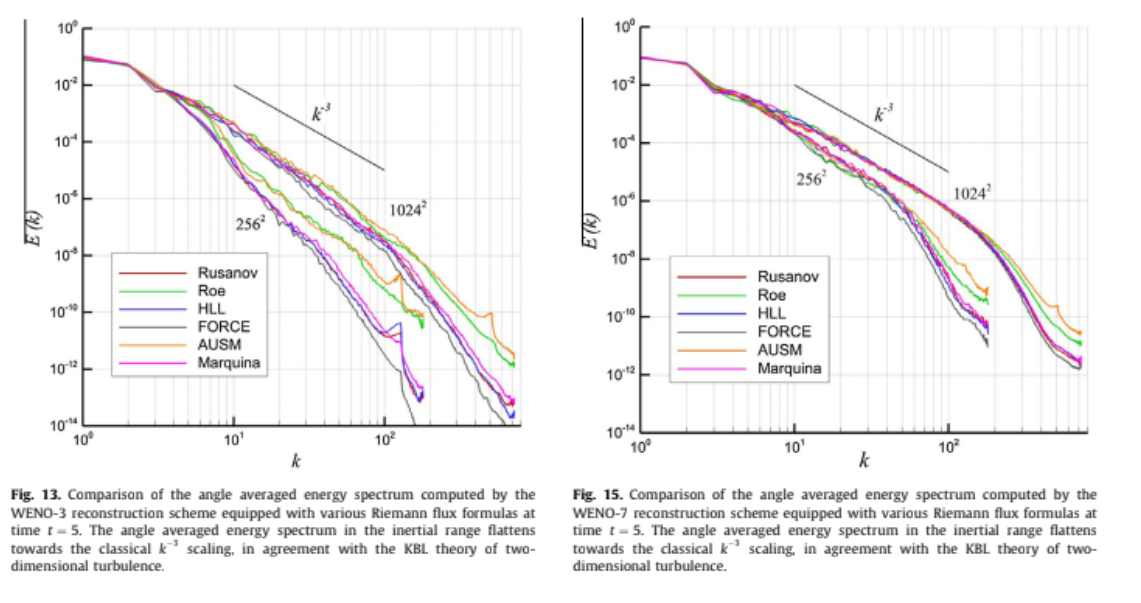
\includegraphics[width=\columnwidth]{ttk11.PNG}
 \caption{ Traitement traditionnel en aéronautique sur l'énergie en fonction du
nombre d'onde.}
 \label{fig:sample}
\end{figure}


\begin{figure}[H]
 \centering % avoid the use of \begin{cener}...\end{center} and use \centering
instead (more compact)
 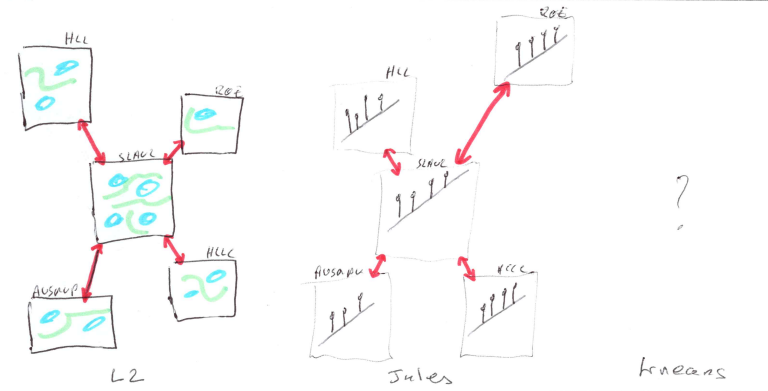
\includegraphics[width=\columnwidth]{ttk2.PNG}
 \caption{Visualisation de la distance L2, les flèches en rouge représentent la
distance entre deux simulation (VTI) à t2(figure de gauche)\\
 Visualisation de la distance topologique, les flèches en rouge représentent la
distance topologique (méthode de Jules) entre deux simulation (Diagrammes de
persistance) à t2(figure du milieu)\\
 Visualisation de la distance topologique, les flèches en rouge représentent la
distance topologique (méthode Kmeans) entre deux simulation (Diagrammes de
persistance) à t2(figure de droite)}
 \label{fig:sample}
\end{figure}


\begin{figure}[H]
 \centering % avoid the use of \begin{center}...\end{center} and use \centering
instead (more compact)
 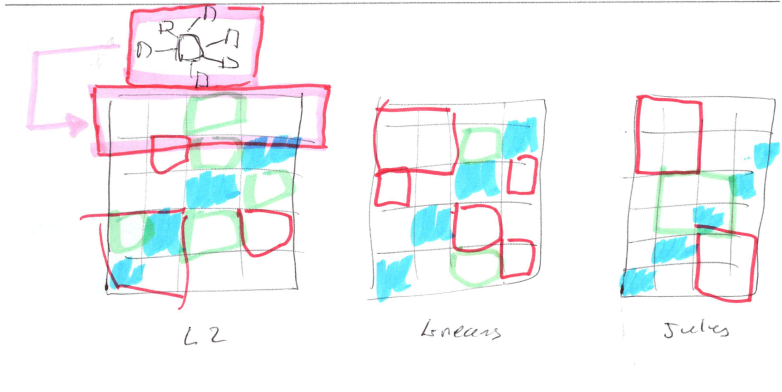
\includegraphics[width=\columnwidth]{ttk3.PNG}
 \caption{Visualisation de la distance L2, les flèches en rouge représentent la
distance entre deux simulation (VTI) à t2(figure en haut à gauche). Matrice de
distance pour la L2 avec les simulations à t2(en bas à gauche). Les carrés en
rouge représentent les clusters de la méthode L2.\\
 Visualisation de la distance topologique, les flèches en rouge représentent la
distance topologique (méthode de Jules) entre deux simulation (Diagrammes de
persistance) à t2(figure en haut du milieu).
 Matrice de distance pour la méthode de Jules avec les simulations à t2(en bas à
gauche). Les carrés en rouge représentent les clusters de la méthode Kmeans.\\
 Visualisation de la distance topologique, les flèches en rouge représentent la
distance topologique (méthode Kmeans) entre deux simulation (Diagrammes de
persistance) à t2(figure en haut à droite).
  Matrice de distance pour la méthode de Jules avec les simulations à t2(en bas
à gauche). Les carrés en rouge représentent les clusters de la méthode de
Jules.\\}
 \label{fig:sample}
\end{figure}


\begin{figure}[H]
 \centering % avoid the use of \begin{center}...\end{center} and use \centering
instead (more compact)
 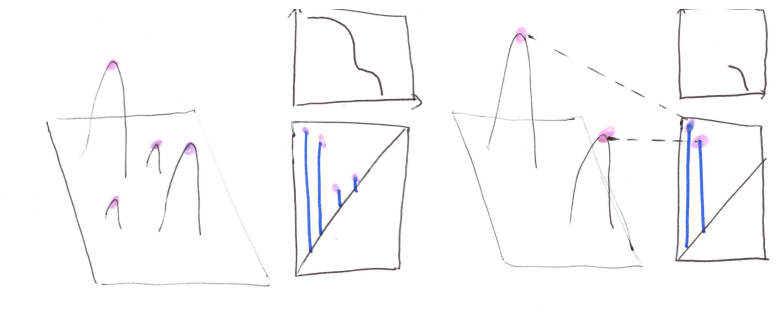
\includegraphics[width=\columnwidth]{ttk4.PNG}
 \caption{Les points critiques en rose sont les maximas. Simulation non filtrée
d'un KHI avec son diagramme de persistance (en bas à gauche) et sa courbe de
persistance (en haut à gauche).\\
 Les points critiques en rose sont les maximas. Simulation filtrée d'un KHI avec
son diagramme de persistance (en bas à droite) et sa courbe de persistance (en
haut à droite).}
 \label{fig:sample}
\end{figure}


\begin{figure}[H]
 \centering % avoid the use of \begin{center}...\end{center} and use \centering
instead (more compact)
 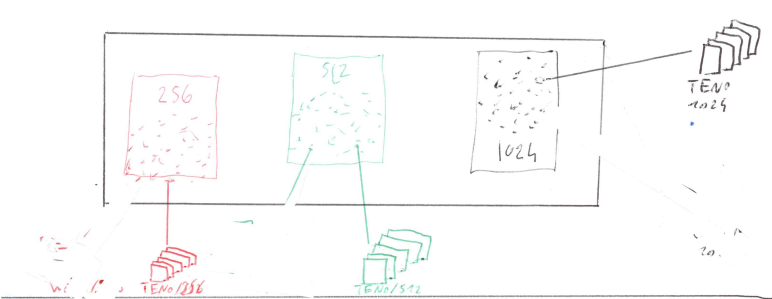
\includegraphics[width=\columnwidth]{ttk7.PNG}
 \caption{Nuage de points (ensemble 60*60), clusterisation par résolution avec
visualisation de certains VTI.}
 \label{fig:sample}
\end{figure}


\begin{figure}[H]
 \centering % avoid the use of \begin{center}...\end{center} and use \centering
instead (more compact)
 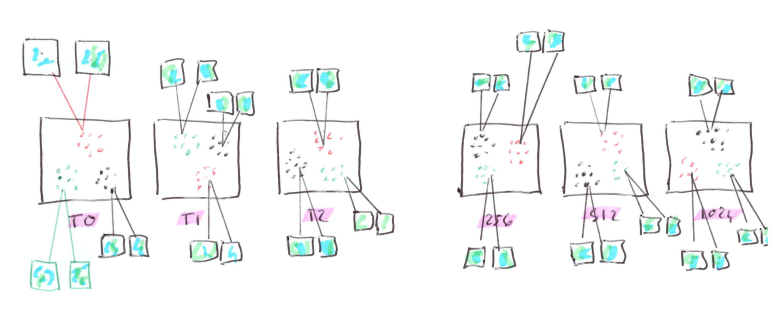
\includegraphics[width=\columnwidth]{ttk6.PNG}
 \caption{Nuage de points à t0,t1 et t2 (ensemble 60*60) avec visualisation de
certains VTI( figure de gauche).\\
 Nuage de points en fonction des résolutions: 256, 512, 1024 (ensemble 60*60)
avec visualisation de certains VTI(figure de droite).}
 \label{fig:sample}
\end{figure}

\begin{figure}[H]
 \centering % avoid the use of \begin{center}...\end{center} and use \centering
instead (more compact)
 \includegraphics[width=\columnwidth]{numerical_study.png}
 \caption{Etude numerique en CFD}
 \label{fig:sample}
\end{figure}


\begin{table}[!ht]
    \centering
    \begin{tabular}{|l|l|l|l|l|}
    \hline
        Schemes & Orders & Meshes & Solvers & Simulation times in seconds \\ \hline
        TENO & 5 & 256*256 & SLAU2 & 140.744 \\ \hline
        TENO & 5 & 256*256 & AUSM$^+$-UP & 212.350 \\ \hline
        TENO & 5 & 256*256 & Roe & 138.090 \\ \hline
        TENO & 5 & 256*256 & HLLC & 216.531 \\ \hline
        TENO & 5 & 256*256 & HLL & 132.921 \\ \hline
        TENO & 5 & 512*512 & SLAU2 & 1235.121 \\ \hline
        TENO & 5 & 512*512 & AUSM$^+$-UP & 786.758 \\ \hline
        TENO & 5 & 512*512 & Roe & 634.823 \\ \hline
        TENO & 5 & 512*512 & HLLC & 1273.546 \\ \hline
        TENO & 5 & 512*512 & HLL & 1119.895 \\ \hline
        TENO & 5 & 1024*1024 & SLAU2 & 10272.841 \\ \hline
        TENO & 5 & 1024*1024 & AUSM$^+$-UP & 5823.188 \\ \hline
        TENO & 5 & 1024*1024 & Roe & 5390.730 \\ \hline
        TENO & 5 & 1024*1024 & HLLC & 5612.924 \\ \hline
        TENO & 5 & 1024*1024 & HLL & 5187.889 \\ \hline
        TENO & 7 & 256*256 & SLAU2 & 189.150 \\ \hline
        TENO & 7 & 256*256 & AUSM$^+$-UP & 185.992 \\ \hline
        TENO & 7 & 256*256 & Roe & 189.150 \\ \hline
        TENO & 7 & 256*256 & HLLC & 267.585 \\ \hline
        TENO & 7 & 256*256 & HLL & 89.920 \\ \hline
        TENO & 7 & 512*512 & SLAU2 & 805.142 \\ \hline
        TENO & 7 & 512*512 & AUSM$^+$-UP & 786.758 \\ \hline
        TENO & 7 & 512*512 & Roe & 1674.321 \\ \hline
        TENO & 7 & 512*512 & HLLC & 773.146 \\ \hline
        TENO & 7 & 512*512 & HLL & 1622.587 \\ \hline
        TENO & 7 & 1024*1024 & SLAU2 & 13165.878 \\ \hline
        TENO & 7 & 1024*1024 & AUSM$^+$-UP & 6779.093 \\ \hline
        TENO & 7 & 1024*1024 & Roe & 6320.002 \\ \hline
        TENO & 7 & 1024*1024 & HLLC & 6491.327 \\ \hline
        TENO & 7 & 1024*1024 & HLL & 6186.092 \\ \hline
        WENO-Z & 5 & 256*256 & SLAU2 & 107.150 \\ \hline
        WENO-Z & 5 & 256*256 & AUSM$^+$-UP & 110.780 \\ \hline
        WENO-Z & 5 & 256*256 & Roe & 108.424 \\ \hline
        WENO-Z & 5 & 256*256 & HLLC & 105.91 \\ \hline
        WENO-Z & 5 & 256*256 & HLL & 98.779 \\ \hline
        WENO-Z & 5 & 512*512 & SLAU2 & 456.877 \\ \hline
        WENO-Z & 5 & 512*512 & AUSM$^+$-UP & 974.777 \\ \hline
        WENO-Z & 5 & 512*512 & Roe & 914.106 \\ \hline
        WENO-Z & 5 & 512*512 & HLLC & 443.987 \\ \hline
        WENO-Z & 5 & 512*512 & HLL & 391.781 \\ \hline
        WENO-Z & 5 & 1024*1024 & SLAU2 & 13165.878 \\ \hline
        WENO-Z & 5 & 1024*1024 & AUSM$^+$-UP & 3977.280 \\ \hline
        WENO-Z & 5 & 1024*1024 & Roe & 3665.727 \\ \hline
        WENO-Z & 5 & 1024*1024 & HLLC & 3844.873 \\ \hline
        WENO-Z & 5 & 1024*1024 & HLL & 3351.741 \\ \hline
        WENO-Z & 7 & 256*256 & SLAU2 & 134.924 \\ \hline
        WENO-Z & 7 & 256*256 & AUSM$^+$-UP & 142.729 \\ \hline
        WENO-Z & 7 & 256*256 & Roe & 127.671 \\ \hline
        WENO-Z & 7 & 256*256 & HLLC & 138.541 \\ \hline
        WENO-Z & 7 & 256*256 & HLL & 123.721 \\ \hline
        WENO-Z & 7 & 512*512 & SLAU2 & 1181.648 \\ \hline
        WENO-Z & 7 & 512*512 & AUSM$^+$-UP & 603.104 \\ \hline
        WENO-Z & 7 & 512*512 & Roe & 547.285 \\ \hline
        WENO-Z & 7 & 512*512 & HLLC & 588.874 \\ \hline
        WENO-Z & 7 & 512*512 & HLL & 516.925 \\ \hline
        WENO-Z & 7 & 1024*1024 & SLAU2 & 10164.932 \\ \hline
        WENO-Z & 7 & 1024*1024 & AUSM$^+$-UP & 10095.930 \\ \hline
        WENO-Z & 7 & 1024*1024 & Roe & 9488.464 \\ \hline
        WENO-Z & 7 & 1024*1024 & HLLC & 9195.901 \\ \hline
        WENO-Z & 7 & 1024*1024 & HLL & 8620.182 \\ \hline
    \end{tabular}
    \caption{Table of simulation times}
\end{table}


% \cleardoublepage
\clearpage
\bibliographystyle{abbrv-doi}
\bibliography{template}
\end{document}

